% !TEX encoding = UTF-8 Unicode
% !TEX spellcheck = en-US


% This is the root file of your thesis: thesis.tex
% A line starting with % is a comment. In some cases, I have included a command preceded by a %. You may activate the command by removing the %.

%%===================================
\documentclass[12pt]{report}
\usepackage{ramsstyle}
\usepackage{wrapfig}
\usepackage[dvipsnames]{xcolor}
\usepackage{todonotes}
\usepackage{enumitem}
% \usepackage[shortlabels]{enumitem}
\usepackage{listings}


\usepackage{caption}
\usepackage{subcaption}
\captionsetup[figure,lstlisting]{font=footnotesize}

\definecolor{codegreen}{rgb}{0,0.6,0}
\definecolor{codegray}{rgb}{0.5,0.5,0.5}
\definecolor{codepurple}{rgb}{0.58,0,0.82}
\definecolor{backcolour}{rgb}{0.95,0.95,0.92}

\definecolor{bluekeywords}{rgb}{0,0,1}
\definecolor{greencomments}{rgb}{0,0.5,0}
\definecolor{redstrings}{rgb}{0.64,0.08,0.08}
\definecolor{xmlcomments}{rgb}{0.5,0.5,0.5}
\definecolor{types}{rgb}{0.17,0.57,0.68}
% \lstdefinestyle{mystyle}{
%     backgroundcolor=\color{backcolour},   
%     commentstyle=\color{codegreen},
%     keywordstyle=\color{magenta},
%     numberstyle=\tiny\color{codegray},
%     stringstyle=\color{codepurple},
%     basicstyle=\ttfamily\footnotesize,
%     breakatwhitespace=false,         
%     breaklines=true,                 
%     captionpos=b,                    
%     keepspaces=true,                 
%     numbers=left,                    
%     numbersep=5pt,                  
%     showspaces=false,                
%     showstringspaces=false,
%     showtabs=false,                  
%     tabsize=2
% }
% \lstset{style=mystyle}
\lstset{language=c++,
captionpos=b,
%numbers=left, %Nummerierung
%numberstyle=\tiny, % kleine Zeilennummern
frame=lines, % Oberhalb und unterhalb des Listings ist eine Linie
basicstyle=\ttfamily\footnotesize,
showspaces=false,
showtabs=false,
breaklines=true,
showstringspaces=false,
breakatwhitespace=false,
numberstyle=\tiny\color{codegray},
numbers = left,
tabsize = 2,
escapeinside={(*@}{@*)},
commentstyle=\color{greencomments},
morekeywords={partial, foreach, var, value, get, set, null, false, true},
keywordstyle=\color{bluekeywords},
stringstyle=\color{redstrings},
}

\setlength{\marginparwidth}{3cm}
\setlength{\parindent}{0pt}
%%===================================
%Write the various parts of your thesis as separate files and include them into the main file by the command \include{name of included file}. When you compile the LaTeX file, you may choose which subfiles to include by the command

%\includeonly{chapter01,chapter02}

%%===================================
\begin{document}
% !TEX encoding = UTF-8 Unicode
%!TEX root = thesis.tex
% !TEX spellcheck = en-US

%This is the Titlepage
%%=========================================
\thispagestyle{empty}

\includegraphics[scale=1.1]{fig/rams}
\mbox{}\\[6pc]
\begin{center}
\Huge{This is the Title of my Thesis}\\[2pc]

\Large{Ole Ravna}\\[1pc]
\large{December 2020}\\[2pc]

PROJECT THESIS\\
Department of Computer Science\\
Norwegian University of Science and Technology
\end{center}
\vfill

\noindent Supervisor 1: Gabriel Kiss 

\noindent Supervisor 2: The co-supervisors (internal and external)

 % This is the titlepage
\setcounter{page}{0}
\pagenumbering{roman}
% % !TEX encoding = UTF-8 Unicode
%!TEX root = thesis.tex
% !TEX spellcheck = en-US
%%=========================================
\addcontentsline{toc}{section}{Preface}
\section*{Preface}


% Something, something...

With this research my time as at NTNU comes to an end. Six years of studies, and more prominently, being a student, has left me inspired and hungry to employ my knowledge to solve real world problems. As such, the thesis before you describes one real world problem and my attempt at solving it.

For this opportunity, I would like to thank my supervisors Ekaterina Prasolova-Førland and Gabriel Kiss, allowing me to pursuit such practical research has been most rewarding. Without fail, Prasolova-Førland has been indispensable both through resources, organizing and her steady support. 
A huge thanks also to Menno P. Witter at the Kavli Institute for bringing forth this problem, for his incredible knowledge of neuroanatomy and most of all for his positivity and humor, every interaction with Witter has been a joy. 
% I would also like to thank all test participants
% When reflecting on the years of studenthood 

During my years as a student I have had the pleasure to meet many new people, two of which have meant much to me and this resulting thesis. First, my girlfriend, Mathilde Theisen, we found each other during a student trip and have during our studies shared an interest for both technology and outdoor activity. And my friend Ask Jentoft, who I met during a summer project where we created our first application using AR technology, and who has sat besides me writing his own master's thesis on medical use of this technology. Many thanks to you both for your help and support, this project would not be complete without you.\\[2cm]


\begin{center}
Trondheim, 24. June 2021 \\[1pc]
\begin{figure}[H]
    \centering
    
\includegraphics[width=0.3\textwidth , trim={0 0 0 0}, clip]{fig/ravnasign}
\end{figure}
% (Your signature)\\[1pc]
Ole Ravna
\end{center}
% % !TEX encoding = UTF-8 Unicode
%!TEX root = thesis.tex
% !TEX spellcheck = en-US
%%=========================================
\addcontentsline{toc}{section}{Acknowledgment}
\section*{Acknowledgment}
I would like to thank the following persons for their great help during \ldots


\begin{flushright}
O.R.\\[1pc]
% (Your initials)
\end{flushright}





% !TEX encoding = UTF-8 Unicode
% !TEX root = thesis.tex
% !TEX spellcheck = en-US
%%=========================================
\addcontentsline{toc}{section}{Executive Summary}
\section*{Abstract}
Something, something...
\tableofcontents
\setcounter{page}{0}
\pagenumbering{arabic}
% !TEX encoding = UTF-8 Unicode
%!TEX root = thesis.tex
% !TEX spellcheck = en-US
%%=========================================
\chapter{Introduction}

%%=========================================

\subsection*{Augmented Reality}

% (Jentoft, 2020) AR can be defined as a system that fulfills three basic features: a combination of real and virtual worlds, real-time interaction, and accurate 3D registration of virtual and real objects.

{
    \color{BrickRed}
    [TODO: Rewrite this shitty part]
    Augmented Reality (AR) describes the use of technology to insert computer generated three-dimensional visuals into the real world in real-time, and the ability to blend interaction between real-world and computer-based objects. 
}
Augmented Reality (AR) describes the use of computer technology to generate an audio-visual experience combining real-world impressions with computer generated graphics, and -essentially- the ability to interact seamlessly between both domains.
 

\noindent Ever since the infancy of AR technology, medical usage has been envisioned as a great potential. The idea of x-ray vision is seen both in science fiction and in genuine research dating all the way back to the 1930s when H. Steinhaus explored ways to visualize metal pieces inside the body \citep{Sielhorst2008}. There is now substantial interest in the use of AR within a wide array of medical fields as well as in industry and education. As an emerging technology there is still much research needed, and great leaps in hardware, software and sensor capabilities are bound to happen in the near future. Already AR shows promising results in both surgical settings and in education \citep{Singh2013}.

\subsection*{Neuroanatomy}

The study of neuroanatomy is concerned with the structural organization of the nervous system. This primarily means the brain and its structures, and that is what this project will focus exclusively on.
Within the study of neuroanatomy, the use of macroscopical brain dissections have long been the conventual practice for teaching the organization of the structures in the brain. Requiring cadavers and the single use of their brain, this method is highly resource intensive and has limited scalability. In addition, there are deeply concerning ethical problems with the use of animals in research. 

\section{Problem Formulation}

%%=========================================
\section{Motivation}

In light of the problems with physical brain dissections it is natural that the use of digital tools, three-dimensional modeling and visualization has been seeing growing use for educational purposes. 
%%=========================================
%%=========================================
According to \citep{Dalgarno2010} computer-aided learning generally increases understanding for anatomy. As anatomy in general, and neuroanatomy specifically are highly complex domains both visually and spatially, the ability to use the human senses in a real-world setting could result in greater intuition and understanding. With that in mind the use of augmented reality could be a natural way to virtualize the experience of a brain dissection, and further the unique capabilities of AR could enable innovative ways of learning. \citep{Moro2017} shows the possibility of greater immersion and engagement while using augmented reality in teaching anatomy to medical students. This has also recently been shown with promising result by  \citep{Wish2020}, where COVID-lockdown required from-home teaching, and the use of HoloAnatomy, an anatomy application for the HoloLens, performed significantly better than even conventional in-class lectures.

%%=========================================
The main problem with most academic implementations, like \citep{Wish2020}, of AR in medical education is the use of head-mounted display (HMD) devices like the HoloLens 2 and Magic Leap, which in the near to mid-term future will have limited practical use in education, as a result of the high price-tag, combined with the still inadequate general use-case for these types of devices.
This project will try to mend these challenges by having the lecturer using an HMD and having student view and interact with the lecture in an AR-based application running on their smartphone. 
%%=========================================
This is possible because of the great leap in AR-performance seen in recent models of Android and especially iPhones, in combination with development platforms like \nameref{chap:unity}, \nameref{chap:mrtk} and \nameref{chap:photon} (see \autoref{chap:tools}) which enables multiplatform development and real-time collaboration between devices. 
% In this pursuit we will also make use of high-resolution 3D imagery of a rat brain (see \autoref{chap:ratbrain}).  
% %%=========================================
\todo[inline]{Introduce Nevrolens and WHS brain}
The aim of the project will be to create a seamless educational experience in Augmented Reality which can be valuable both on an HMD device and a modern smartphone. The focus will be on investigating its feasibility as an educational tool both in a lecture-type setting and for students to explore the brain anatomy independently. 

%%==========================================




%%=========================================
\subsection*{What Remains to be Done?}

%%=========================================
\section{Objectives / Research Questions}
What follow are the research questions which motivates this project: \\
\noindent
\textbf{Main RQ:} How can AR support teaching of rat brain anatomy and dissection for medical students?
\begin{itemize}
    \item {
        \textbf{Sub-RQ1:} How should interaction in be implemented in AR to accommodate medical professionals?
    }
    \item {
        \textbf{Sub-RQ2:} How will a collaborative experience shared between an HMD and a smartphone compare to accommodate medical professionals?
    }
    {
        \newline
        \color{BrickRed}
        \textbf{Sub-RQ3: }
        Something about macro + microscopic visualization, some suggestions:
        \item Can microscopical data seamlessly be integrated into a macroscopical model? 

        \item Can understanding be increased by integrating microscopical data into a macroscopical model?

        \item Will having integrated microscopical data in a macroscopical model lead to greater understanding?
    }
\end{itemize}


%%=========================================
\section{Approach}


\subsection*{Research method}

\begin{wrapfigure}{R}{0.50\textwidth}
    \begin{center}
        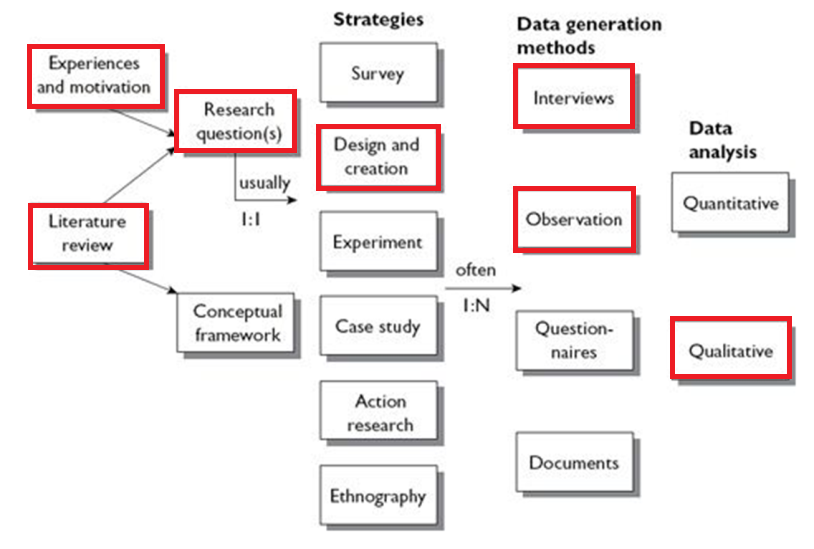
\includegraphics[width=0.42\textwidth]{fig/researchplan_image}
    \end{center}
    \caption{Model of the research process as illustrated in \citet{oates2006} }
    \label{researchplan_img}
\end{wrapfigure}

The research questions were derived through discussing the needs of the intended users with neuroscientists at the Kavli Institute. It was then narrowed down by a literature review, finding a lack of satisfactory substitutions for real brain dissections and especially finding no attempt at a practical multiplatform application for a more scalable use for students. The projects research question falls under the strategy of Design and Creation as the main goal is to develop a useful application for medical education. The focus on a smartphone solution was further motivated by the COVID-pandemic making from-home learning quite essential and making the passing around of HMD devices an unwanted scenario. As part of an agile software development model the gathering of qualitative data from observations and interviews within the scope of user testing will be essential. 

\subsection*{Development method}

\section{Contributions}
%% write about macro vs micro stuff

The research product resulting from this project will be a new computer-based software application using augmented reality and running on multiple platforms like HoloLens 1 and 2, Android and more. The aim will be to develop an application that can bridge the gap between expensive head mounted displays and everyday smartphones which you will find in the pocket of any student, and to use this as a collaborative tool for learning neuroanatomy. Throughout the development period we will consult with medical professionals and gather feedback from students on the usability of the application.

{
    \color{BrickRed}
    \noindent
    \newline
    Something about macro + micro
}

%%=========================================
\section{Limitations}

%%=========================================
\section{Outline}


\include{chapters/Background}
\chapter{Requirements}\label{chap:req}


% \section{Requirements}

% cadavers difficult to get, vr -> less awareness
%
%


The first meeting initializing the project took place at VRLab Dragvoll in early September, here I was introduced to the general background and the problem description of how Witter and others envisioned the use of AR for neuroanatomical education. It was explained how cadavers for education are difficult to acquire and therefore used quite sparingly. 
Another problem we discussed was related to the difference in medium between VR and AR. While the application \nameref{chap:vrvis} did have many of the features envisioned, and could have been a basis for further development. The fact that is was implemented in VR was problematic for the envisioned use cases. Being completely enclosed visually limits its use case in lectures and in any use case with collaboration in a physical space. Generally the loss of spatial awareness and eye contact as a result of using VR headsets was though of as an impediment for using VR for such an application. 
% something about the data set?
Thus, we had an outline of a neuroanatomical education tool in AR using the HoloLens 2 and concluded with some questions and requirements for the project:

\begin{enumerate}\label{mennoslist}
    \item Can the current VR dataset\footnotemark be used in the HoloLens 2 AR environment?
    \item If not, which steps need to be taken to use the segmented WHS rat brain to develop a suitable 3D model that can be used in AR?
    \item Develop an optimal user interface for a single person to explore the rat brain as if the user is doing a dissection of a real brain.
    \item Develop/test ways to make this a multiuser/shareable tool adequate in a teaching environment.
    \item Explore ways to integrate microscopical data into the AR representation.
    \item Describe/explore the feasibility to implement the system for Human neuroanatomy education.
\end{enumerate}

\footnotetext{Referring to \nameref{chap:vrvis} by \citep{Elden2017}.}

Here items 1-4 were deemed critical for the project, while 5 and 6 were dependent on the progress made.

This meeting together with the list formed a clear problem description and can be seen as the initial discovery process of the project. Though the following period of exploring the newly arrived HoloLens 2 and its capabilities, we formed a set of \textit{system requirements}. 
System requirements are descriptions of how a system should operate, what it should be able to do and the constraints of its operation. The requirements must reflect the stakeholders needs for the system \citep{PUboka}. System requirements are generally split into functional requirements, which describe specifics of what the system (and its sub-systems) should do, and non-functional requirements, which generally are descriptions of the user experience of the system as a whole. 
What follows are the system requirements decided on for the application: 

\subsection*{Functional Requirements}
\begin{enumerate}
    \item {
        \textbf{Implement a brain dissection tool in AR.}\\
        The app should render a brain at sufficient quality for educational use, and have the tools for creating a dissection experience in AR.
        
    }
    \item {
        \textbf{The application must run in HoloLens 2 and at least one mobile platform}\\
        The ability to run a version for the app on multiple platforms is essential for the purpose of this project. While the main platforms are HoloLens and mobile, others may also be implemented in the future. 
    }

    \item {
        \textbf{Implement cross-platform collaboration over network}\\
        For the application to have value above a single user it is important that it can be used with a HoloLens and a more accessible platforms in a collaborative manner. 
    }


\end{enumerate}

\subsection*{Non-Functional Requirements}

\begin{enumerate}
    \item {
        \textbf{Medical students should find educational use for the app.}\\
        It is critical that there is educational value in the application. 
    }
    \item {
        \textbf{The application should be usable without outside guidance.}\\
        The app should have a clear and understandable design, such that a new user should be able to navigate the app by them self, even with minimal experience with AR.
    }
    \item {
        \textbf{All relevant usability criteria for a mixed reality app should be met.}\\
We should work to not fall under the 'meets' criteria on any relevant metric in the App quality criteria\footnote{https://docs.microsoft.com/en-us/windows/mixed-reality/develop/platform-capabilities-and-apis/app-quality-criteria}. This includes criteria on; FPS, spatial anchoring and view comfort. 
    }
\end{enumerate}
\chapter{Technical Design}\label{chap:techdesign}

This chapter will give a overview of the structure of the application as well as some choices taken when developing the research product, Nevrolens. The chapter will exclusively focus on the application as it is at the end of this research project, which is functionally identical to version 0.3.3 of Nevrolens. However, some refactoring i.e. name changes and restructuring may have occurred. 

\section{Game Structure}

\subsection*{Unity Scene Graph}

Within Unity a \textit{Scene} consists of a \textit{scene graph} which is a tree structure of \texttt{GameObjects}. By default a scene consist of a \texttt{Directional Light} lighting up the scene at its default light source and a \texttt{Main Camera} which is the view point of the running game. In addition, the MRTK library will add two objects to the scene graph, one called \texttt{MixedRealityToolkit} which contains configuration of the Mixed Reality features and systems. This is where input systems are defined and where control of spatial awareness and boundary detection is handled, in short all features and sensors of the HoloLens system or other AR system are defined and controlled here. The other object added by MRTK is the \texttt{MixedRealityPlayspace}, this encapsulates the \texttt{Main Camera}, but is lacking any useful documentation on what its purpose is. The name could be hinting at it being the parent of the \textit{Playspace}, meaning all \texttt{GameObjects} in the game. However, even MRTK demos seem to ignore this object and thus it has not been used in this project either.

The functionality of the scene graph, other than organizing GameObjects, is that child objects inherit the position, rotation and scale of their parents, thus simplifying transformation of complex object. This naturally structures many systems, however in a AR application there can be many independent 3D objects floating in space. In addition, some objects are dependent not on their parent, but on a defined object \texttt{Transform}. Therefore, some organization is needed and some objects are placed by choice and convenience rather than any practical reason. Another practical use for child objects are the use of the \texttt{GameObject.GetComponentsInChildren()} and \texttt{GameObject.GetComponentInParent()} methods which allows for simple access to \texttt{Components} in child and parent \texttt{GameObjects}, this is however of limited use as such dependencies in code has a tendency to result in tedious bugs.

The top most application specific object of the project is the \texttt{BrainSystem}, this acts as the parent GameObject for all objects defined by the application. The right side of \autoref{fig:brainsystem} gives an overview of all 3D object in the \texttt{BrainSystem}. The \texttt{InfoBoard} on the right, the button group, or \texttt{HandMenu} in the center and the complete brain model with axes etc. named \texttt{GameWorldSpace}, are spatially independent systems all having \texttt{BrainSystem} as a parent, this can also be seen in \autoref{fig:brainsystem} in the scene hierarchy on the left side. The reasoning for having the parent object \texttt{BrainSystem} is purely to to tidy up the top layer of the scene graph and having a clear distinction of project specific custom objects. 

The main attraction within the \texttt{BrainSystem} is the \texttt{GameWorldSpace}, it is the parent of the brain model and all objects with are spatially dependent on the brain. This allows for movement and scaling of the whole model worldspace. This is also the local space of the synchronized multiplayer world. 

% notice that the blue "black board" on the right, the button group and the brain are independent spatially.

\begin{figure}[ht]
    \centering
    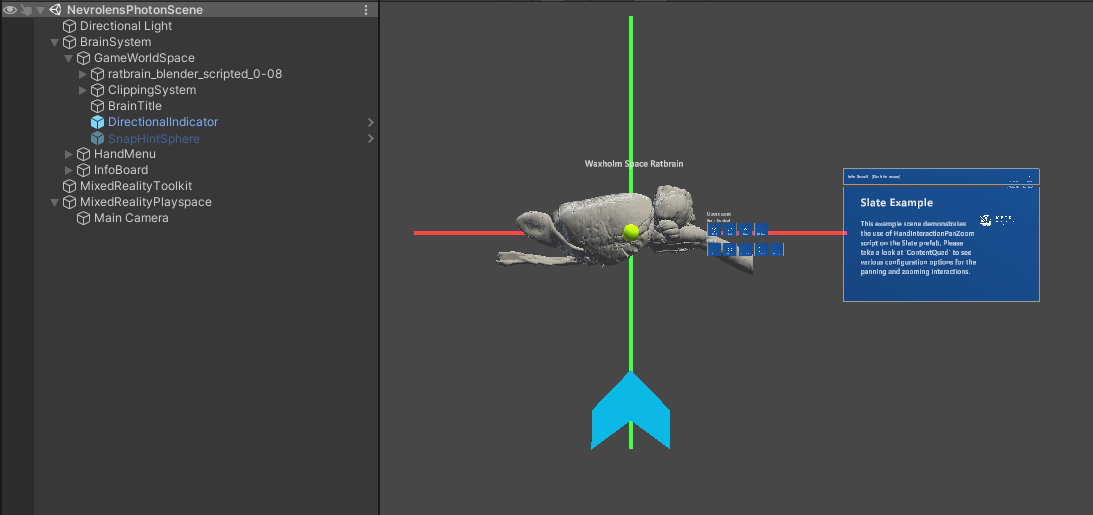
\includegraphics[width=\textwidth]{fig/brainsystemoverview5.png}
    \caption{Every 3D object in the \texttt{BrainSystem}}
    \label{fig:brainsystem}
\end{figure}
% In general there is few limitations on how to structure the scene graph, its functionality other than structural,

\section{Networking}

\subsection*{Networking Solutions}

Multiplayer games in Unity can be created in numerous ways, in the development phase of this project three solutions were explored; UNET,  LiteNetLib and Photon PUN2 . Common for all are that they are mature, reliable and are well documented, they all support multiple device types including all devices within the scope of this project, there are however some very clear differences making the choice for this project quite simple.
% mlapi, mirror, playfab
\textit{UNET} is Unity's own default networking solution, it provides high level functionality and is generally easy to use. It is however deprecated and will be discontinued by the end of 2021, an open source fork of the networking API, called \textit{Mirror} has seen continuing development and improvement, but because of the state of the original project, both were deemed nonideal. Unity is working on a new networking solution called \textit{MLAPI}, it is in alpha stages but shows great promise.

\textit{LiteNetLib} is a open source, and more low level framework. It is intended for use cases where in-depth control of the networking processer are wanted or needed, if high performance and low latency is important this would be a good choice. It supports peer-to-peer and self-managed servers. Because this project can be thought of a small scale proof of concept, it is of limited concern whether the networking is highly performant and seeing as a low level API is more complicated to implement it is neither a optimal use of a single developers time.

Lastly, \textit{Photon PUN2} is the an high level networking library with managed hosting and a free basic plan for up till 20 concurrent users. This makes it ideal for small projects and single developers. It is also the general first choice for networking solution in Unity and its surge in popularity is partly the reason for Unity abandoning their own solution. PUN2 was a natural choice simply because is of its low barrier for entry and it having a free hosting options making development as easy as possible. It being the most popular solution also has the added benefit of having well made tutorials and forums for troubleshooting.

While developing this application, Microsoft announced a new solution for networking specifically targeting MR applications called \textit{Microsoft Mesh}, it promises to solve networking, and many MR specific problems like spatial anchoring and face-to-face interaction. This could be a promising step for this application in the projects continuation, and should be kept an eye on by future researchers.

\subsection*{Connection}

\begin{wrapfigure}[14]{r}{0.4\textwidth} 
    \centering
    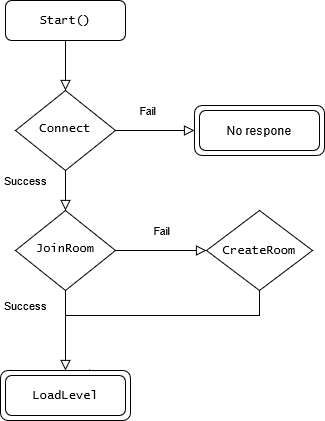
\includegraphics[width=0.3\textwidth]{fig/photonconnectiondiagram2.png}
    \caption{State diagram of the implemented connection process}
    \vspace{30pt}
    \label{fig:photonconnect}
\end{wrapfigure}
In this project, networking has as stated been implemented as simply as possible for a proof of concept and because of time constraints on a single developer. If concerns like scalability and reliability was of higher importance different choices would have been made, and steps to fulfill those concerns should probably be taken in future development.
When using the networking, which is how the built versions of the application are set up, the application initially launches in a empty \texttt{Scene} named \texttt{NevrolensStartPhotonScene}, its only purpose is connecting the user to the server and creating or joining a \textit{room}. A room is a Photon abstraction for connecting users to the same game state. \autoref{item:photonconnect} shows a striped down version of the script running in this scene, it is a complete and functional script to emphasize the ease of implementation. The script  is all that is needed to initiate a connation in Photon PUN2, and is all connection handling in the application. The implementation has, because of its simplicity, some flaws, \autoref{fig:photonconnect} shows that if connection to the photon server fails the application will give no response and the user will just stay in an empty scene, this could easily be fixed by either giving some error message feedback with a retry button or even loading the game scene in offline mode, neither has been implement mainly because connation issues have seldom raised and thus development time has not been invested in fixing this problem. 

\begin{lstlisting}[language=c, label={item:photonconnect}, caption={The connect process in a Unity \texttt{MonoBehaviour} written in C\#. }]
    void Start() {
        PhotonNetwork.ConnectUsingSettings();
    }
    override void OnConnectedToMaster() {
        PhotonNetwork.JoinRandomRoom(); 
    }
    override void OnJoinRandomFailed(short returnCode, string msg) {
        PhotonNetwork.CreateRoom(roomName: "room1"); 
    }
    override void OnJoinedRoom() {
        if (PhotonNetwork.IsMasterClient)
            PhotonNetwork.LoadLevel("NevrolensPhotonScene");
    }
\end{lstlisting}

Another implication of this design is that every user will necessarily connect to the same room. This happens because the first user will find no room and thus create a new one, while all others will find the one room and connect to it. The user has no control over who they play with, and can not start a session by them self, both could easily be implemented, but would also result in overhead for the user as they will have to make a choice which now is simply made for them.

All in all this solution work well enough for the current state of the research project. In fact, by abstracting away the connection and room selection process it has simplified the user testing process because there are fewer steps to get to a running application. 


\begin{figure}
    \centering
    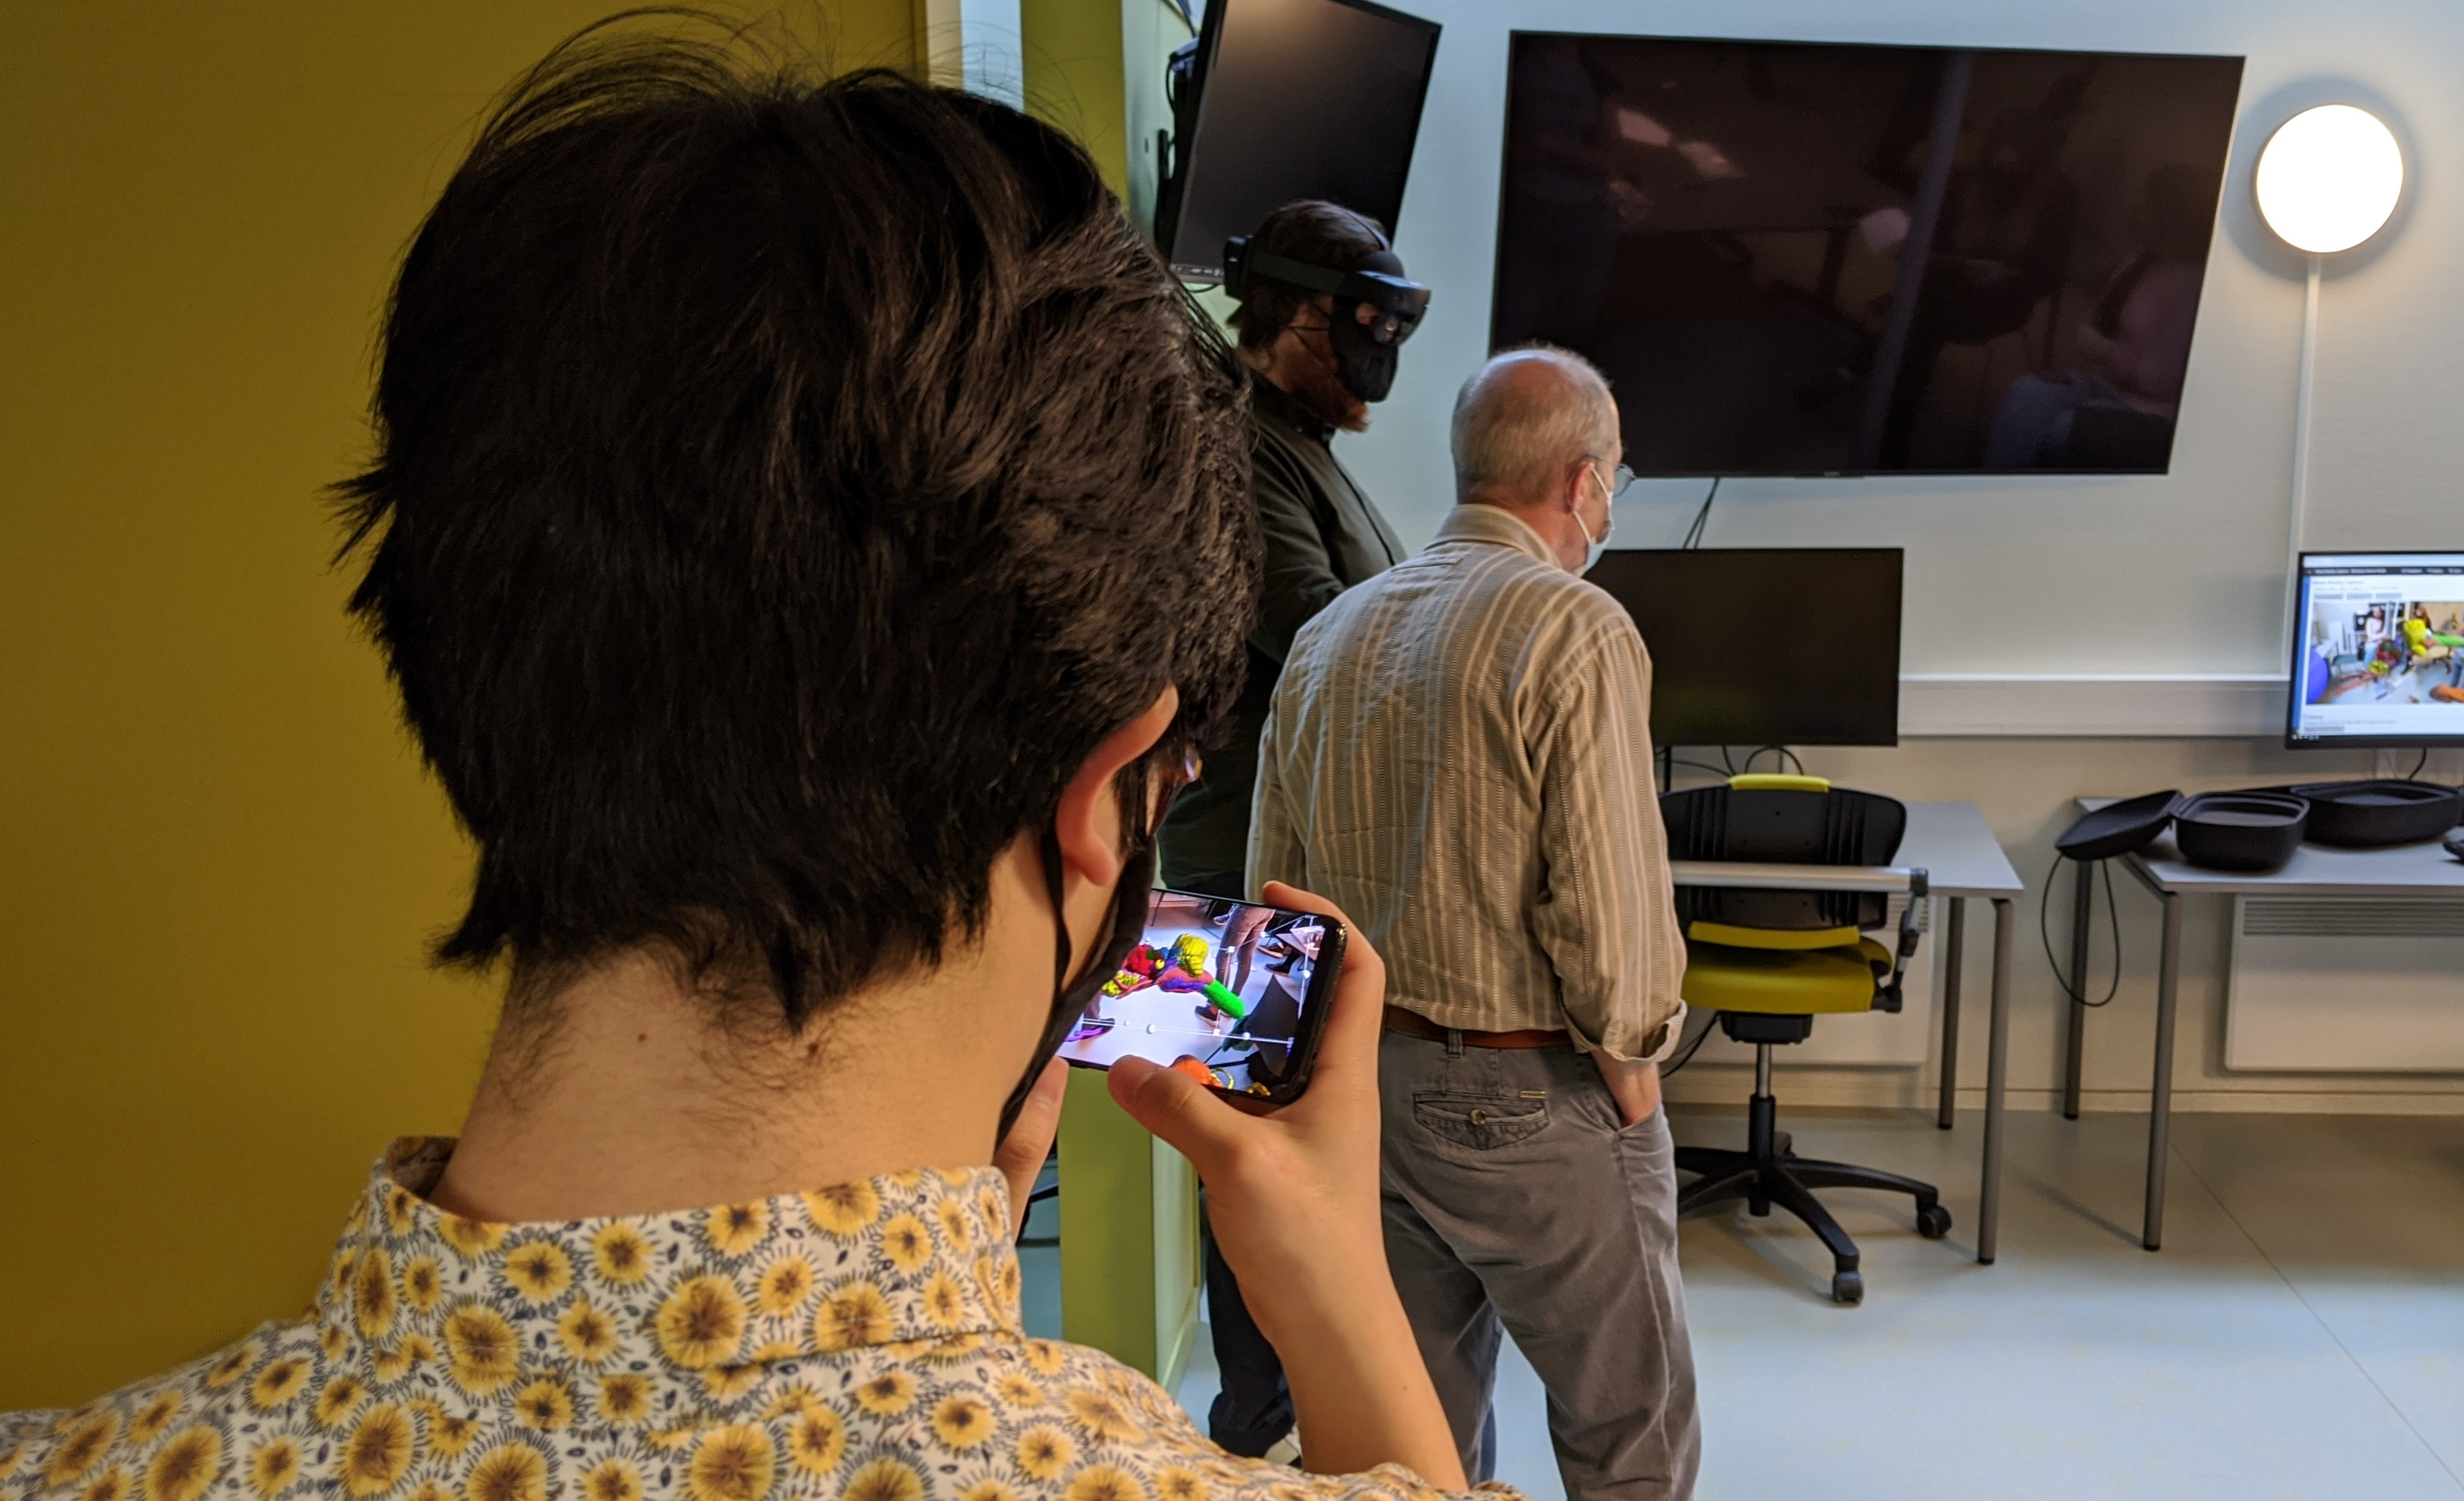
\includegraphics[width=0.8\textwidth]{fig/nevrolensandroidtester.jpg}
    \caption{Networking allows the Android test user to see the same brain model as the HoloLens 2 user. The monitor on the background displays a live feed from the HoloLens device.}
\end{figure}

\subsection*{Multiplayer world space}\label{chap:multiplayerworldspace}
% local world space, multiplay space, rotation etc

When collaborating with other players there is a need for having a synchronized world space, by default Photon PUN2 will synchronize all objects spatially by their own model space, or \texttt{local space}. This works good for basic tasks like synchronize the movement of a brain structure relative to the others, but meets problems when separating the shared multiplayer world space from from the local user world space. This is needed so that a user can move the AR objects to fit in their field of view, physical surroundings and at the scale appropriate for their comfort and device type. For this reason all GameObjects which are to be synchronized in the shared multiplayer world space are placed as children of an empty GameObject called \texttt{GameWorldSpace} and the local model space of this object is used as the multiplayer world space. With this implementation, and manipulation of the \texttt{GameWorldSpace} is local and not shared over network, while any manipulation of its child object will be reflected for all users over the network. 

\chapter{Development Process}


\section{Software Process}
% https://www.wikipendium.no/TDT4140_Programvareutvikling/nb/#kapittel-2-software-processes

% Incremental development etc. \#agile
% \large{Where everything I learned in PU should shine!}

Even though the software process in developing the Nevrolens application has been done by a single developer, effort has been made to use best practices for a software development workflow. These practices have generally grown out of the the needs of a multi-developer setting, enabling simpler use of collaboration and version control. Though their value possibly increases exponentially by the number of team members, the developer has found value in the structure and clarity found in the workflow. 

\begin{figure}[h]
    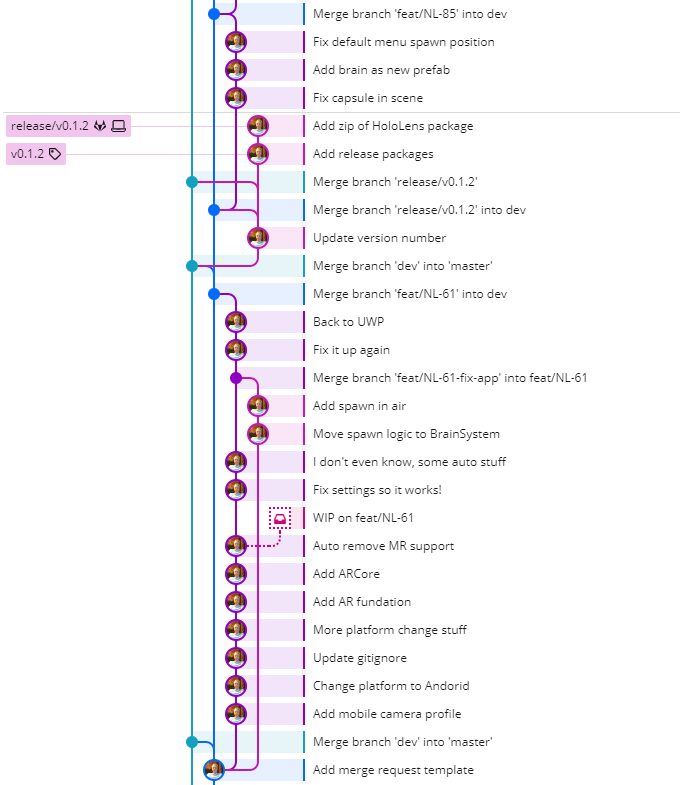
\includegraphics[width=0.33\textwidth]{fig/gitkraken_gitlog}
    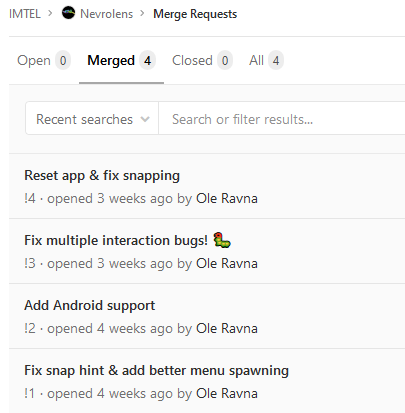
\includegraphics[width=0.33\textwidth]{fig/mergerequests}
    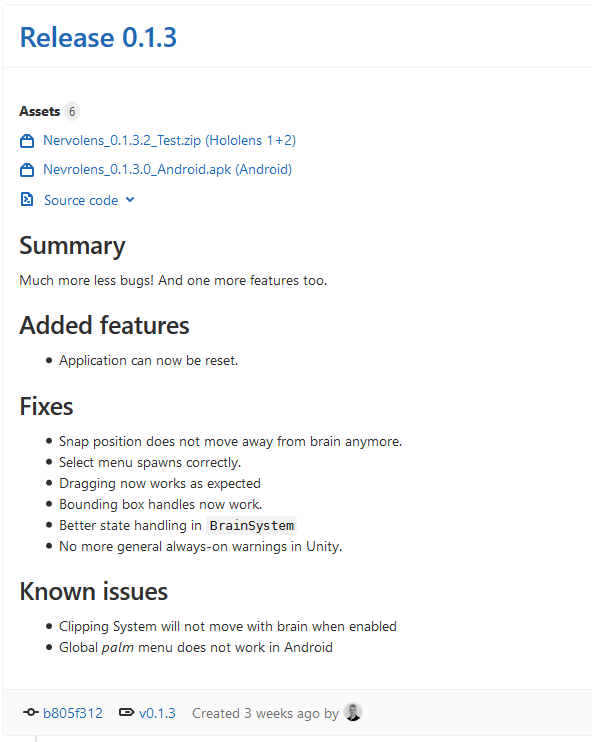
\includegraphics[width=0.33\textwidth]{fig/release_gitlab}
    \caption{Feature branches, merge requests and releases.}
\end{figure}

The workflow is based on \textit{Gitflow}, a workflow framework optimized for continuous software development. In short, this is just a very basic rule set for branch-naming and the sanctity of the master-branch (requiring merge requests of only product ready code), within the version control system \nameref{chap:git}. It does however act as a fundament which enables practices like rapid release cycles, because of the clearly define production ready state, and the integration with lean development technics like Kanban. This stems from the parallels between feature-branches in Gitflow and the \textit{ticket} in Kanban. In practice, this means that tickets, with issues or new features for the app, are created on in the \textit{Backlog} column of the Kanban board and are then moved to \textit{Doing} column simultaneously as a feature-branch is created with the ID of the ticket, e.g. \texttt{feat/NL-42}. All of this is automated in the Git management tool \nameref{chap:gitkraken}, which manages both the git-repo and the Kanban board.

\begin{figure}[h]
    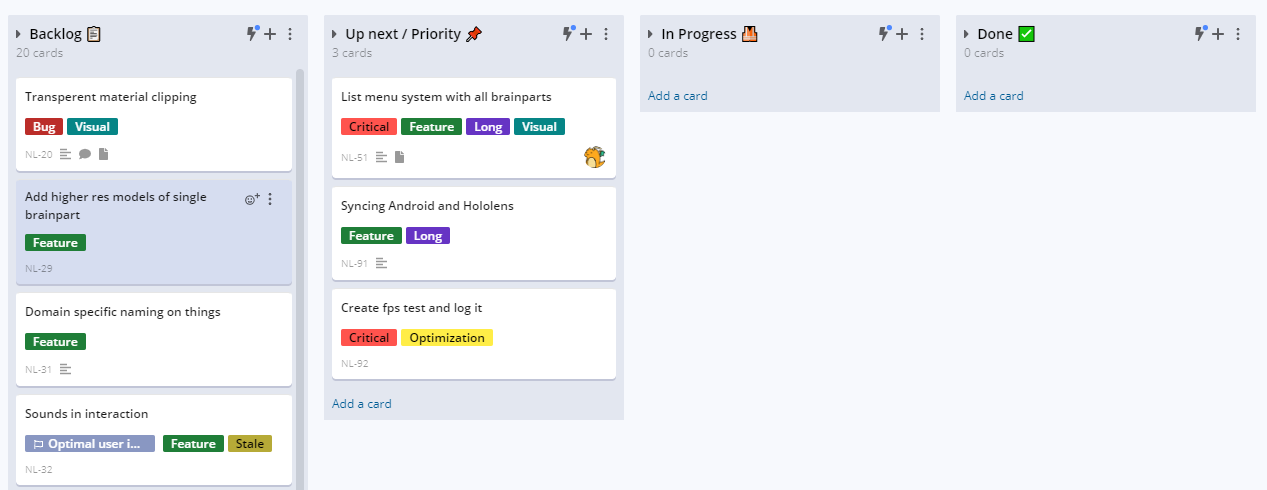
\includegraphics[width=\textwidth]{fig/kanban2}
    \caption{A snapshot of the Kanban board in GitKraken, after a development sprint, when completed tickets are archived (closed).\\ Note: \textit{Priority} acts as pined tickets on \textit{Backlog}, as the backlog tends to sizeable.}
    \label{fig:kanban}
\end{figure}

This workflow, by design, supports an agile development process. Agile approaches to software development are generally human-centered, valuing individuals and interactions over processes and tools\footnote{The Agile Manifesto https://agilemanifesto.org/}, and focused on iterating rather than upfront planning. This is ideas which are beneficial for single-developer or small teams especially when developing for new platforms like the HoloLens 2. 
While the project aims for an agile approach, the sprint cycle core to the agile development, where stakeholders are involved for regular feedback, has, due to a number of factors like COVID-19, only really been done for one cycle. However, the steps taken for an agile workflow should enable more agile development for the master project.

% One thing that I have not incorporated in to the workflow is user stories. The tickets in \autoref{fig:kanban} are written only for my understanding and will seem confusing and untidy for others. By using the concept of user stories 

% and will limited testing possibilities due to COVID-19 


% this enables me as a developer to test the product rapidly against users. 
% , this means having rules for branch naming, creating merge requests when merging to the `master`-branch, and 
% !TEX encoding = UTF-8 Unicode
% !TEX root = ../thesis.tex
% !TEX spellcheck = en-US
%%=========================================



\chapter{Implementation}

% Hololens, UWP, WMR

\section{Requirements}

% cadavers difficult to get, vr -> less awareness
%
%


The first meeting initializing the project took place at VRLab Dragvoll in early September, here I was introduced to the general background and the problem description of how Witter and others envisioned the use of AR for neuroanatomical education. It was explained how cadavers for education are difficult to acquire and [\dots]. 
Another problem we discussed was related to the difference in medium between VR and AR. While the application \nameref{chap:vrvis} did have many of the features envisioned, and could have been a basis for further development. The fact that is was implemented in VR was problematic for the envisioned use cases. Being completely enclosed visually limits its use case in lectures and in any use case with collaboration in a physical space. Generally the loss of spatial awareness and eye contact as a result of using VR headsets was though of as an impediment for using VR for such an application. 
% something about the data set?
Thus, we had an outline of a neuroanatomical education tool in AR using the HoloLens 2 and concluded with some questions and requirements for the project:

\begin{enumerate}\label{mennoslist}
    \item Can the current VR dataset\footnotemark be used in the HoloLens 2 AR environment?
    \item If not, which steps need to be taken to use the segmented WHS rat brain to develop a suitable 3D model that can be used in AR?
    \item Develop an optimal user interface for a single person to explore the rat brain as if the user is doing a dissection of a real brain.
    \item Develop/test ways to make this a multiuser/shareable tool adequate in a teaching environment.
    \item Explore ways to integrate microscopical data into the AR representation.
    \item Describe/explore the feasibility to implement the system for Human neuroanatomy education.
\end{enumerate}

\footnotetext{Referring to \nameref{chap:vrvis}.}

Here items 1-4 were deemed critical for the project, while 5 and 6 were dependent on the progress made.

This meeting together with the list formed a clear problem description and can be seen as the initial discovery process of the project. Though the following period of exploring the newly arrived HoloLens 2 and its capabilities, we formed a set of \textit{system requirements}. 
System requirements are descriptions of how a system should operate, what it should be able to do and the constraints of its operation. The requirements must reflect the stakeholders needs for the system \citep{PUboka}. System requirements are generally split into functional requirements, which describe specifics of what the system (and its sub-systems) should do, and non-functional requirements, which generally are descriptions of the user experience of the system as a whole. 
What follows are the system requirements decided on for the application: 

\subsection*{Functional Requirements}
\begin{enumerate}
    \item {
        \textbf{Implement a brain dissection tool in AR}\\
         
    }
    \item {
        \textbf{The application must run in HoloLens 2 and a mobile platform}\\
         Android and/or iOS
    }

    \item {
        \textbf{Collaboration}\\
         
    }

\end{enumerate}

\subsection*{Non-Functional Requirements}

\begin{enumerate}
    \item 
\end{enumerate}

% and non-functional requirements, which describe  










\section{Software Process}
% https://www.wikipendium.no/TDT4140_Programvareutvikling/nb/#kapittel-2-software-processes

% Incremental development etc. \#agile
\large{Where everything I learned in PU should shine!}

Even though I have developed the Nevrolens application by myself, I have strived to use best practices for a software development workflow. These practices have generally grown out of the the needs of a multi-developer setting, to simplify the needs for collaboration and version control. Though their value possibly increases exponentially by the number of team members, I have found value in the structure and clarity I find in the workflow. 
My workflow consist of 




\section{Validation / Testing}



\chapter{Deployment}

The application in this research has been development using Microsoft's Mixed Reality Toolkit and has followed the platforms best practices and recommendations. The deployment process for HoloLens devices are based on sideloading of the application compiled and built with Visual Studio Community 2019, this is the standard way of both building and deploying for HoloLens. For Android the principle of sideloading is also used, but here Unity is responsible for compilation and the build process. 
The application as 


\subsection*{Installation of Nevrolens}

This section will be a guide for installing Nevrolens on HoloLens 2 and Android from packages hosted on GitLab.
By following the instructions for HoloLens 2, this should also work for HoloLens 1, but has limited testing on that platform as it was not a focus of this research.

\subsubsection*{Deploy to HoloLens 2}

\begin{enumerate}
    \item {
        \textbf{Go to the release page}\\
        Found here: \url{https://gitlab.stud.idi.ntnu.no/olevra/nevrolens/-/releases}
    }
    \item {
        \textbf{Choose a release}\\
        Preferably the topmost and latest. This research ends on is version 0.3.3. 
    }

    \item {
        \textbf{Download the HoloLens zip package}\\
        Under \textit{Packages} click on the package for HoloLens (1 and 2) to download it.
    }

    \item {
        \textbf{Unzip file}\\
        Open the downloaded ZIP-file and extract it.
    }

    \item {
        \textbf{Open the Windows Device Portal for HoloLens}\\
        Guide by Microsoft: \href{https://docs.microsoft.com/en-us/windows/mixed-reality/develop/platform-capabilities-and-apis/using-the-windows-device-portal}{Using the Windows Device Portal}
    }
    \item {
        \textbf{Install appxbundle}\\
        Under \textit{Views / Apps} click \texttt{Choose File} and locate the APPXBUNDLE-file inside the folder extracted from the ZIP-file. Then click \texttt{Install}.
    }

\end{enumerate}

\subsubsection*{Deploy to Android}

\begin{enumerate}
    \item {
        \textbf{Go to the release page on your Android device}\\
        Found here: \url{https://gitlab.stud.idi.ntnu.no/olevra/nevrolens/-/releases}
    }
    \item {
        \textbf{Choose a release}\\
        Preferably the topmost and latest. This research ends on is version 0.3.3. 
    }

    \item {
        \textbf{Download the Android APK-file}\\
        Under \textit{Packages} click on the package for Android to download it.
    }

    \item {
        \textbf{Open the downloaded file.}\\
        Your device will ask for your permission to install an application from a unknown source. Accepting this, the device will start installing the application.
    }

\end{enumerate}

\subsection*{Getting started with developing the project}
This section will briefly explain how to set up the project for development, this differs from deployment in that the goal is to be able to continue development of the project from within Unity and with supporting tools. This is the process the current developer uses when developing from a new computer.
Having completed this set up deployment of the application can be done, directly from Unity for Android and through Visual Studio 2019 for HoloLens devices.


\textbf{Requirements}
\begin{enumerate}
    \item Git and Git LFS
    \item { Unity 2019.4 LTS \\
    When installing add: \textit{Android Build support} }
    \item {Visual Studio 2019 \\
    When installing add: \textit{Universal Windows Platform development}, \textit{USB Device Connectivity}, \textit{Game development with Unity} }
\end{enumerate}
Begin by cloning the \textit{Git} repository by typing: \\ \texttt{git clone https://gitlab.stud.idi.ntnu.no/olevra/nevrolens.git} in to \textit{Git Bash}, than type \texttt{git lfs install \&\& git lfs fetch \-\-all}. Now open Unity Hub and locate and add the repository just cloned as a Unity project. Open it with Unity 2019.4, it is critical that this version is used for MRTK to work properly. First time opening this project will take some time, when it is done the project is ready.
% The deployment process can be found in MRTK documentation 
\chapter{Testing}


This chapter will explore how testing has been accomplished in this research project, both day-to-day software testing, but also feedback from stakeholders and formal user testing. Because of the current COVID-19 pandemic, physical meeting and user testing been done sparingly, and have at times been impossible carry out, in fact the fall semester did not see any physical testing by users not affiliated with the VRLab at NTNU Dragvoll.

\section{Software testing}
During development, software testing has been done unstructured, mostly by way of regular deployment and on-device feature testing. This is admittedly not the most comprehensive testing system and can not guarantee intended behavior as systems are combined and restructured, in the same way as a test suit with \textit{unit testing} and \textit{integration testing} could. But it allows for more rapid development, less overhead for a single developer and can not be said to have meaningfully limited the research project. A case could be made for a testing suit being helpful in the continuation of the research as new developers will have a concrete indication of intended behavior, this has and could not have a high priority as a development goal, because of limitations in development time and the demand for creating a research result.

\section{Stakeholder meetings}


\section{User Testing}
% !TEX encoding = UTF-8 Unicode
%!TEX root = thesis.tex
% !TEX spellcheck = en-US
%%=========================================



\chapter{Results}\label{chap:results}




The results in this research project are mainly gathered from the final test session, which was held after the last development stage, thus the results reflect the state of the application at the end of the research. 

The test sessions had two separate qualitative data gathering strategies: 

A multiple choice knowledge test taken by the test participants before and after the session,  this was meant to demonstrate learning value in short term time frame. Such a simple short term test could support the claim that the artifact can be used as an educational tool. The test is attached as \autoref{chap:knowtest}.
The second strategy was a combined SUS questionnaire with general questions about the application. This questionnaire can be found as \autoref{chap:questionnaire}.
The knowledge test was taken by the medical students in test sessions, while the questionnaire was answered by six participants, of which four were medical students.

% though further research is needed.

\section{Neuroanatomical test}
The multiple choice neuroanatomical knowledge test was performed at both test sessions. The test was taken by three medical students at the first session, two third year and one fifth year student. At the second session five first year medical students partook in the knowledge test.

\begin{figure}[H]
    \centering
    \begin{subfigure}[t]{0.8\textwidth}
        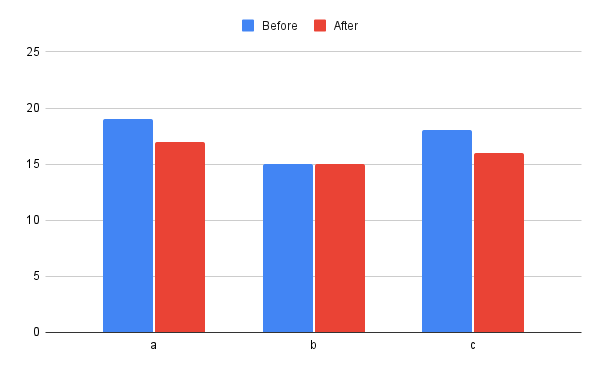
\includegraphics[width=\textwidth]{fig/knowtestresult1}
        \caption{}
    \end{subfigure}
    \begin{subfigure}[b]{0.8\textwidth}
        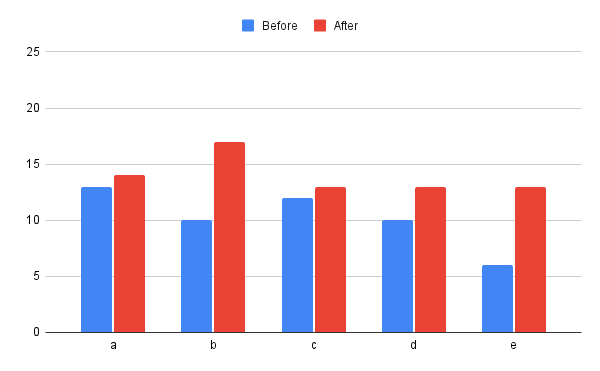
\includegraphics[width=\textwidth]{fig/knowtestresult2}
        \caption{}
    \end{subfigure}
\end{figure}





\section{Questionnaire}

The usability results are based on the second test session where a questionnaire, including a SUS section, was uses in addition to unstructured feedback from the test participants. The results from these methods will be presented in this section. 

\subsection{System usability scale questionnaire}
 
The SUS questionnaire was taken by six participants, five answering based on the HoloLens 2 experience and one based on using the Android application. The mean score from the HoloLens 2 is $79.0 \pm 10.4$, while the result from the single Android test was 75. This means that the application on HoloLens 2 sits high in the good rating almost reaching excellent, while the Android app is near the middle of the good rating. \autoref{fig:susresults} show the results of the SUS questionnaire charted with the red line representing the 68 \textit{average} score. All answers are listed in \autoref{tab:sus}, note that SUS is ordered such that every other statement is negative, meaning that a better score is achieved when they are disagreed to.

% Please add the following required packages to your document preamble:
% \usepackage[table,xcdraw]{xcolor}
% If you use beamer only pass "xcolor=table" option, i.e. \documentclass[xcolor=table]{beamer}
\begin{table}[]
    
\centering
\textbf{Results from SUS questionnaire}\par\medskip
\small
\begin{tabular}{l|ccccc}
\hline
                                                                                                                                         & \begin{tabular}[c]{@{}c@{}}Strongly\\ disagree\end{tabular} & Disagree                                                   & Neutral                                                    & Agree                                                     & \begin{tabular}[c]{@{}c@{}}Strongly\\ agree\end{tabular}   \\ \hline
\begin{tabular}[c]{@{}l@{}}I think that I would like to use this \\ system frequently.\end{tabular}                                      & {\color[HTML]{333333} \textbf{}}                            & {\color[HTML]{333333} \textbf{}}                           & {\color[HTML]{333333} \textbf{}}                           & \cellcolor[HTML]{9698ED}{\color[HTML]{EFEFEF} \textbf{2}} & \cellcolor[HTML]{6434FC}{\color[HTML]{EFEFEF} \textbf{4*}} \\
\rowcolor[HTML]{EFEFEF} 
\begin{tabular}[c]{@{}l@{}}I found the system \\ unnecessarily complex.\end{tabular}                                                     & \cellcolor[HTML]{6665CD}{\color[HTML]{EFEFEF} \textbf{3}}   & \cellcolor[HTML]{9698ED}{\color[HTML]{EFEFEF} \textbf{2*}} & \cellcolor[HTML]{CBCEFB}{\color[HTML]{EFEFEF} \textbf{1}}  & {\color[HTML]{333333} \textbf{}}                          & {\color[HTML]{333333} \textbf{}}                           \\
\begin{tabular}[c]{@{}l@{}}I thought the system was \\ easy to use.\end{tabular}                                                         & {\color[HTML]{333333} \textbf{}}                            & {\color[HTML]{333333} \textbf{}}                           & \cellcolor[HTML]{9698ED}{\color[HTML]{EFEFEF} \textbf{2*}} & \cellcolor[HTML]{6434FC}{\color[HTML]{EFEFEF} \textbf{4}} & {\color[HTML]{333333} \textbf{}}                           \\
\rowcolor[HTML]{EFEFEF} 
\begin{tabular}[c]{@{}l@{}}I think that I would need the \\ support of a technical person \\ to be able to use this system.\end{tabular} & \cellcolor[HTML]{6665CD}{\color[HTML]{EFEFEF} \textbf{3*}}  & \cellcolor[HTML]{9698ED}{\color[HTML]{EFEFEF} \textbf{2}}  & \cellcolor[HTML]{CBCEFB}{\color[HTML]{EFEFEF} \textbf{1}}  & {\color[HTML]{333333} \textbf{}}                          & {\color[HTML]{333333} \textbf{}}                           \\
\begin{tabular}[c]{@{}l@{}}I found the various functions in \\ this system were well integrated.\end{tabular}                            & {\color[HTML]{333333} \textbf{}}                            & {\color[HTML]{333333} \textbf{}}                           & \cellcolor[HTML]{CBCEFB}{\color[HTML]{EFEFEF} \textbf{1*}} & \cellcolor[HTML]{6434FC}{\color[HTML]{EFEFEF} \textbf{4}} & \cellcolor[HTML]{CBCEFB}{\color[HTML]{EFEFEF} \textbf{1}}  \\
\cellcolor[HTML]{EFEFEF}\begin{tabular}[c]{@{}l@{}}I thought there was too much \\ inconsistency in this system.\end{tabular}            & \cellcolor[HTML]{CBCEFB}{\color[HTML]{EFEFEF} \textbf{1}}   & \cellcolor[HTML]{6665CD}{\color[HTML]{EFEFEF} \textbf{3}}  & \cellcolor[HTML]{CBCEFB}{\color[HTML]{EFEFEF} \textbf{1}}  & \cellcolor[HTML]{CBCEFB}{\color[HTML]{EFEFEF} \textbf{1*}}   & \cellcolor[HTML]{EFEFEF}\textbf{}                          \\
\begin{tabular}[c]{@{}l@{}}I would imagine that most \\ people would learn to use \\ this system very quickly.\end{tabular}              & {\color[HTML]{333333} \textbf{}}                            & {\color[HTML]{333333} \textbf{}}                           & \cellcolor[HTML]{CBCEFB}{\color[HTML]{EFEFEF} \textbf{1}}  & \cellcolor[HTML]{6665CD}{\color[HTML]{EFEFEF} \textbf{3}} & \cellcolor[HTML]{9698ED}{\color[HTML]{EFEFEF} \textbf{2*}} \\
\rowcolor[HTML]{EFEFEF} 
\begin{tabular}[c]{@{}l@{}}I found the system very \\ cumbersome to use.\end{tabular}                                                    & \cellcolor[HTML]{9698ED}{\color[HTML]{EFEFEF} \textbf{2}}   & \cellcolor[HTML]{6665CD}{\color[HTML]{EFEFEF} \textbf{3}}  & \cellcolor[HTML]{CBCEFB}{\color[HTML]{EFEFEF} \textbf{1*}} & {\color[HTML]{333333} \textbf{}}                          & {\color[HTML]{333333} \textbf{}}                           \\
\begin{tabular}[c]{@{}l@{}}I felt very confident using \\ the system.\end{tabular}                                                       & {\color[HTML]{333333} \textbf{}}                            & {\color[HTML]{333333} \textbf{}}                           & \cellcolor[HTML]{CBCEFB}{\color[HTML]{EFEFEF} \textbf{1}}  & \cellcolor[HTML]{9698ED}{\color[HTML]{EFEFEF} \textbf{2}} & \cellcolor[HTML]{6665CD}{\color[HTML]{EFEFEF} \textbf{3*}} \\
\rowcolor[HTML]{EFEFEF} 
\begin{tabular}[c]{@{}l@{}}I needed to learn a lot of \\ things before I could get \\ going with this system.\end{tabular}               & \cellcolor[HTML]{9698ED}{\color[HTML]{EFEFEF} \textbf{2*}}  & \cellcolor[HTML]{6665CD}{\color[HTML]{EFEFEF} \textbf{3}}  & {\color[HTML]{333333} \textbf{}}                           & \cellcolor[HTML]{CBCEFB}{\color[HTML]{EFEFEF} \textbf{1}} & {\color[HTML]{333333} \textbf{}}                           \\ \hline
\end{tabular}
\caption{The results form the SUS section. Number and color values represent the magnitude of answers with the corresponding alternative. Android answer is marked with "*".}
\label{tab:sus}

\end{table}

\begin{figure}
    \centering
    \textbf{SUS results}\par\medskip
    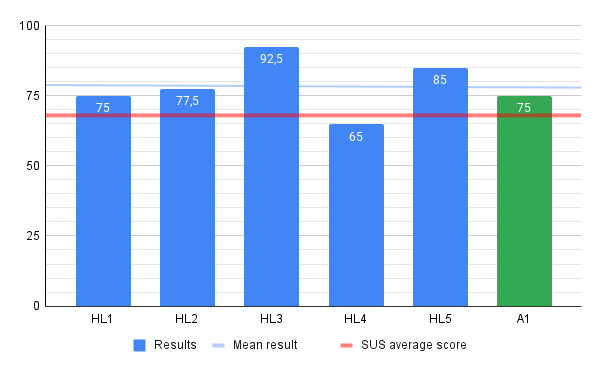
\includegraphics[width=0.75\textwidth]{fig/susbarchart}
    \caption{The blue results are from HoloLens 2, while the green is from Android.}
    \label{fig:susresults}
\end{figure}


\subsection{Research specific questionnaire}\label{chap:researchspes}
The questionnaire included a section with research specific questions written by the researcher with the aim to gather data relating to the research questions of the project. The question were, just as in SUS, based on the \textit{Likert scale}, with answer alternatives ranging from 1 - 5 indicating how much in agreement the user is with the statement. The section was answered by six participants, and it was platform independent. The results can be seen in \autoref{tab:researchspes}. In addition to the Likert ranking free form text boxes were provided after the questions for gathering qualitative data. 


% Notably, the participants were asked what platform they preferred
Notably, every participant who tried both platforms preferred the HoloLens 2 experience, based on the question \textit{Which platform did you prefer?}. Saying the following:
\newline
\textbf{Why did you prefer that platform?}
{\small\itshape
\begin{itemize}[]
    \item Physically interactive and the menu is on your hand
    \item Much easier to understand the 3d structure, as you can see and rotate it at any angle.
    \item Holo is easier to manoeuvre and look from different angles.
    \item It was more a more fun way of learning, which again increases motivation for learning.
\end{itemize}
}

% Please add the following required packages to your document preamble:
% \usepackage[table,xcdraw]{xcolor}
% If you use beamer only pass "xcolor=table" option, i.e. \documentclass[xcolor=table]{beamer}
% \usepackage[normalem]{ulem}
% \useunder{\uline}{\ul}{}
\begin{table}[h]
\centering
\textbf{Results from research questionnaire}\par\medskip
\small
\begin{tabular}{l|ccccc}
\hline
                                                                                                                                                          & \begin{tabular}[c]{@{}c@{}}Strongly\\ disagree\end{tabular} & Disagree                                                  & Neutral                                                   & Agree                                                     & \begin{tabular}[c]{@{}c@{}}Strongly\\ agree\end{tabular}  \\ \hline
\begin{tabular}[c]{@{}l@{}}I got new insight about neuroanatomy \\ while using the system.\end{tabular}                                                   & \textbf{}                                                   & \textbf{}                                                 & \textbf{}                                                 & \cellcolor[HTML]{6434FC}{\color[HTML]{EFEFEF} \textbf{4}} & \cellcolor[HTML]{9698ED}{\color[HTML]{EFEFEF} \textbf{2}} \\
\rowcolor[HTML]{EFEFEF} 
\begin{tabular}[c]{@{}l@{}}I got new insight about neuroanatomy \\ while seeing and manipulating the \\ brain and its structures in 3D.\end{tabular}      & \textbf{}                                                   & \textbf{}                                                 & \textbf{}                                                 & \cellcolor[HTML]{9698ED}{\color[HTML]{EFEFEF} \textbf{2}} & \cellcolor[HTML]{6434FC}{\color[HTML]{EFEFEF} \textbf{4}} \\
\begin{tabular}[c]{@{}l@{}}I got new insight about neuroanatomy \\ while dissecting the brain.\end{tabular}                                               & \textbf{}                                                   & \textbf{}                                                 & \cellcolor[HTML]{CBCEFB}{\color[HTML]{EFEFEF} \textbf{1}} & \cellcolor[HTML]{6200C9}{\color[HTML]{EFEFEF} \textbf{5}} & \textbf{}                                                 \\
\rowcolor[HTML]{EFEFEF} 
\cellcolor[HTML]{EFEFEF}\begin{tabular}[c]{@{}l@{}}I felt like I was collaborating with another \\ person when using the system with others.\end{tabular} & \cellcolor[HTML]{CBCEFB}{\color[HTML]{EFEFEF} \textbf{1}}                           & \cellcolor[HTML]{CBCEFB}{\color[HTML]{EFEFEF} \textbf{1}}                         & \cellcolor[HTML]{6665CD}{\color[HTML]{EFEFEF} \textbf{3}} & \cellcolor[HTML]{CBCEFB}{\color[HTML]{EFEFEF} \textbf{1}}                         & \cellcolor[HTML]{EFEFEF}\textbf{}                         \\
\begin{tabular}[c]{@{}l@{}}I was aware of what the other person did \\ and had focus on when using the system.\end{tabular}                               & \textbf{}                                                   & \cellcolor[HTML]{9698ED}{\color[HTML]{EFEFEF} \textbf{2}} & \cellcolor[HTML]{6665CD}{\color[HTML]{EFEFEF} \textbf{3}} & \cellcolor[HTML]{CBCEFB}{\color[HTML]{EFEFEF} \textbf{1}} & \textbf{}                                                 \\
\rowcolor[HTML]{EFEFEF} 
\begin{tabular}[c]{@{}l@{}}The system would be useful for remote \\ teaching of neuroanatomy.\end{tabular}                                                & \textbf{}                                                   & \textbf{}                                                 & \cellcolor[HTML]{CBCEFB}{\color[HTML]{EFEFEF} \textbf{1}} & \cellcolor[HTML]{9698ED}{\color[HTML]{EFEFEF} \textbf{2}} & \cellcolor[HTML]{6665CD}{\color[HTML]{EFEFEF} \textbf{3}} \\ \hline
\end{tabular}
\caption{The results form the research specific questions, the number and color values represent the magnitude of answers with the corresponding alternative.}
\label{tab:researchspes}
\end{table}

\subsection{IPEAR AR and peer learning questionnaire}
This section was included as part of other research at the NTNU VRLab. The results from the section is however just as relevant for this study. \autoref{tab:peer} shows the results.

\begin{table}[]
\centering
\textbf{Results from AR and peer learning questionnaire}\par\medskip
\small
\begin{tabular}{l|ccccc}
\hline
                                                                                                                                             & \begin{tabular}[c]{@{}c@{}}Strongly\\ disagree\end{tabular} & Disagree                                                  & Neutral                                                   & Agree                                                     & \begin{tabular}[c]{@{}c@{}}Strongly\\ agree\end{tabular}  \\ \hline
\begin{tabular}[c]{@{}l@{}}Did you like the approach of peer learning \\ \small{(working with and teaching your classmates)}?\end{tabular}           & \textbf{}                                                   & \textbf{}                                                 & \cellcolor[HTML]{6665CD}{\color[HTML]{EFEFEF} \textbf{3}} &  & \cellcolor[HTML]{6665CD}{\color[HTML]{EFEFEF} \textbf{3}} \\
\rowcolor[HTML]{EFEFEF} 
\begin{tabular}[c]{@{}l@{}}Were you more interested in teaching \\each other  and sharing content with \\your peers and AR tools?\end{tabular} & \textbf{}                                                   & \cellcolor[HTML]{CBCEFB}{\color[HTML]{EFEFEF} \textbf{1}} & \cellcolor[HTML]{CBCEFB}{\color[HTML]{EFEFEF} \textbf{1}} & \cellcolor[HTML]{6434FC}{\color[HTML]{EFEFEF} \textbf{4}} & {\color[HTML]{EFEFEF} \textbf{}}                          \\
\begin{tabular}[c]{@{}l@{}}Did this learning approach make you feel \\ more responsible for your learning?\end{tabular}                      & \textbf{}                                                   & \cellcolor[HTML]{CBCEFB}{\color[HTML]{EFEFEF} \textbf{1}} & \cellcolor[HTML]{6665CD}{\color[HTML]{EFEFEF} \textbf{3}} & \cellcolor[HTML]{CBCEFB}{\color[HTML]{EFEFEF} \textbf{1}} & \cellcolor[HTML]{CBCEFB}{\color[HTML]{EFEFEF} \textbf{1}} \\
\rowcolor[HTML]{EFEFEF} 
\begin{tabular}[c]{@{}l@{}}Do you think it would be useful in other \\ courses or fields of study as well?\end{tabular}                      & {\color[HTML]{EFEFEF} \textbf{}}                            & {\color[HTML]{EFEFEF} \textbf{}}                          & {\color[HTML]{EFEFEF} \textbf{}}                          & \cellcolor[HTML]{9698ED}{\color[HTML]{EFEFEF} \textbf{2}} & \cellcolor[HTML]{6434FC}{\color[HTML]{EFEFEF} \textbf{4}} \\ \hline
\end{tabular}
\caption{The results form the research specific questions, the number and color values represent the magnitude of answers with the corresponding alternative.}
\label{tab:peer}
\end{table}


\subsection{Feedback from participants}

During the test sessions the participants gave feedback on their thoughts of the application, and how to improve the user experience. For the HoloLens 2 application the stated feedback was overwhelmingly positive, in \autoref{chap:researchspes} some give more constructive feedback which was not pointed out when talking with the participants. For the Android experience the prime vocalized feedback was to disable the AR in the application such that it would be a standard 3D application, this was explained both by the poor spatial locking on the device and the non optimal ergonomics of having to point the camera on the same spot at all times. 





%====================================================

% % The result of this project is the preliminary work for my master thesis next semester, thus 

% \section{Nevrolens}\label{nevrolens}
% Nevrolens is the name I've given the application which is the research product of this project. It's a combination of the Norwegian word Nevroanatomi and HoloLens. It is a AR application running on HoloLens 1, HoloLens 2 and Android. 

% The application is focused on delivering a single user experience, with features as cutting planes, scaling, moving brain parts and transparent brain parts. \autoref{fig:nevrolens_holo} show these features running on HoloLens 2, while \autoref{fig:nevrolens_android} show them on Android.
% It is packages and released on GitLab at \url{https://gitlab.stud.idi.ntnu.no/imtel/nevrolens}. 

% \begin{figure}[h]\label{fig:nevrolens_holo}
%     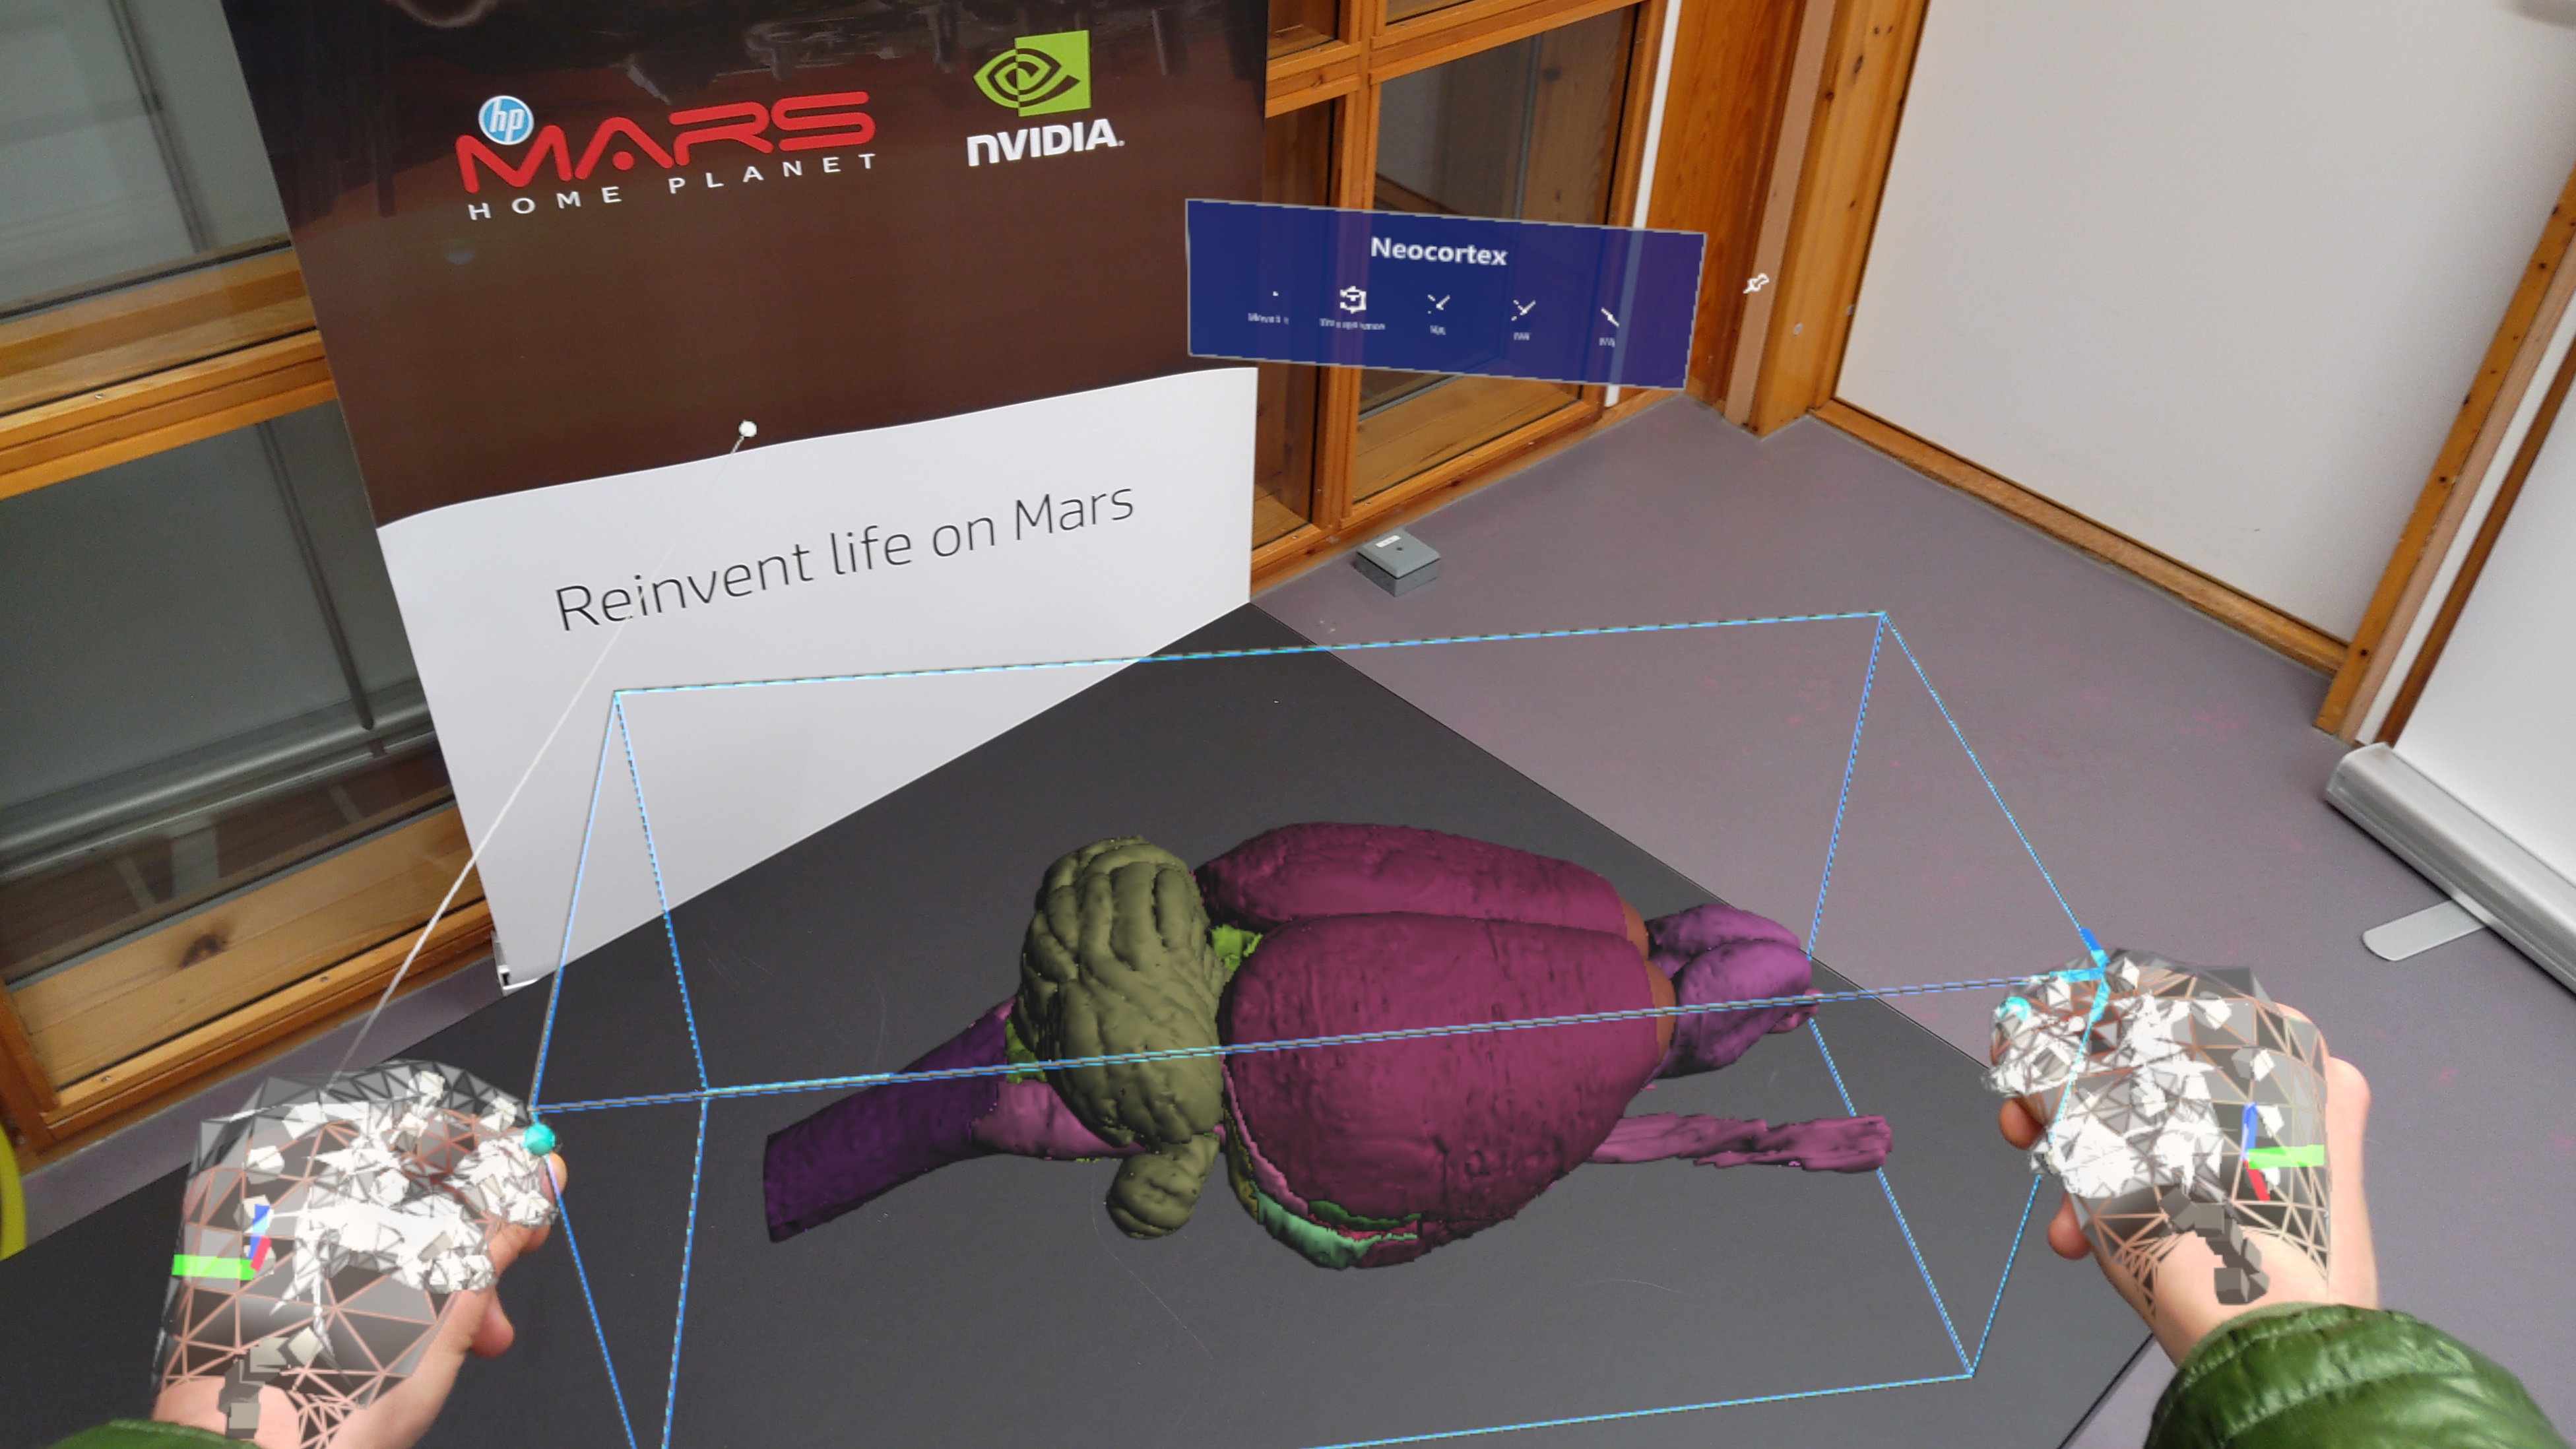
\includegraphics[width=0.5\textwidth]{fig/nevrolens/twohandedzoom.jpg}
%     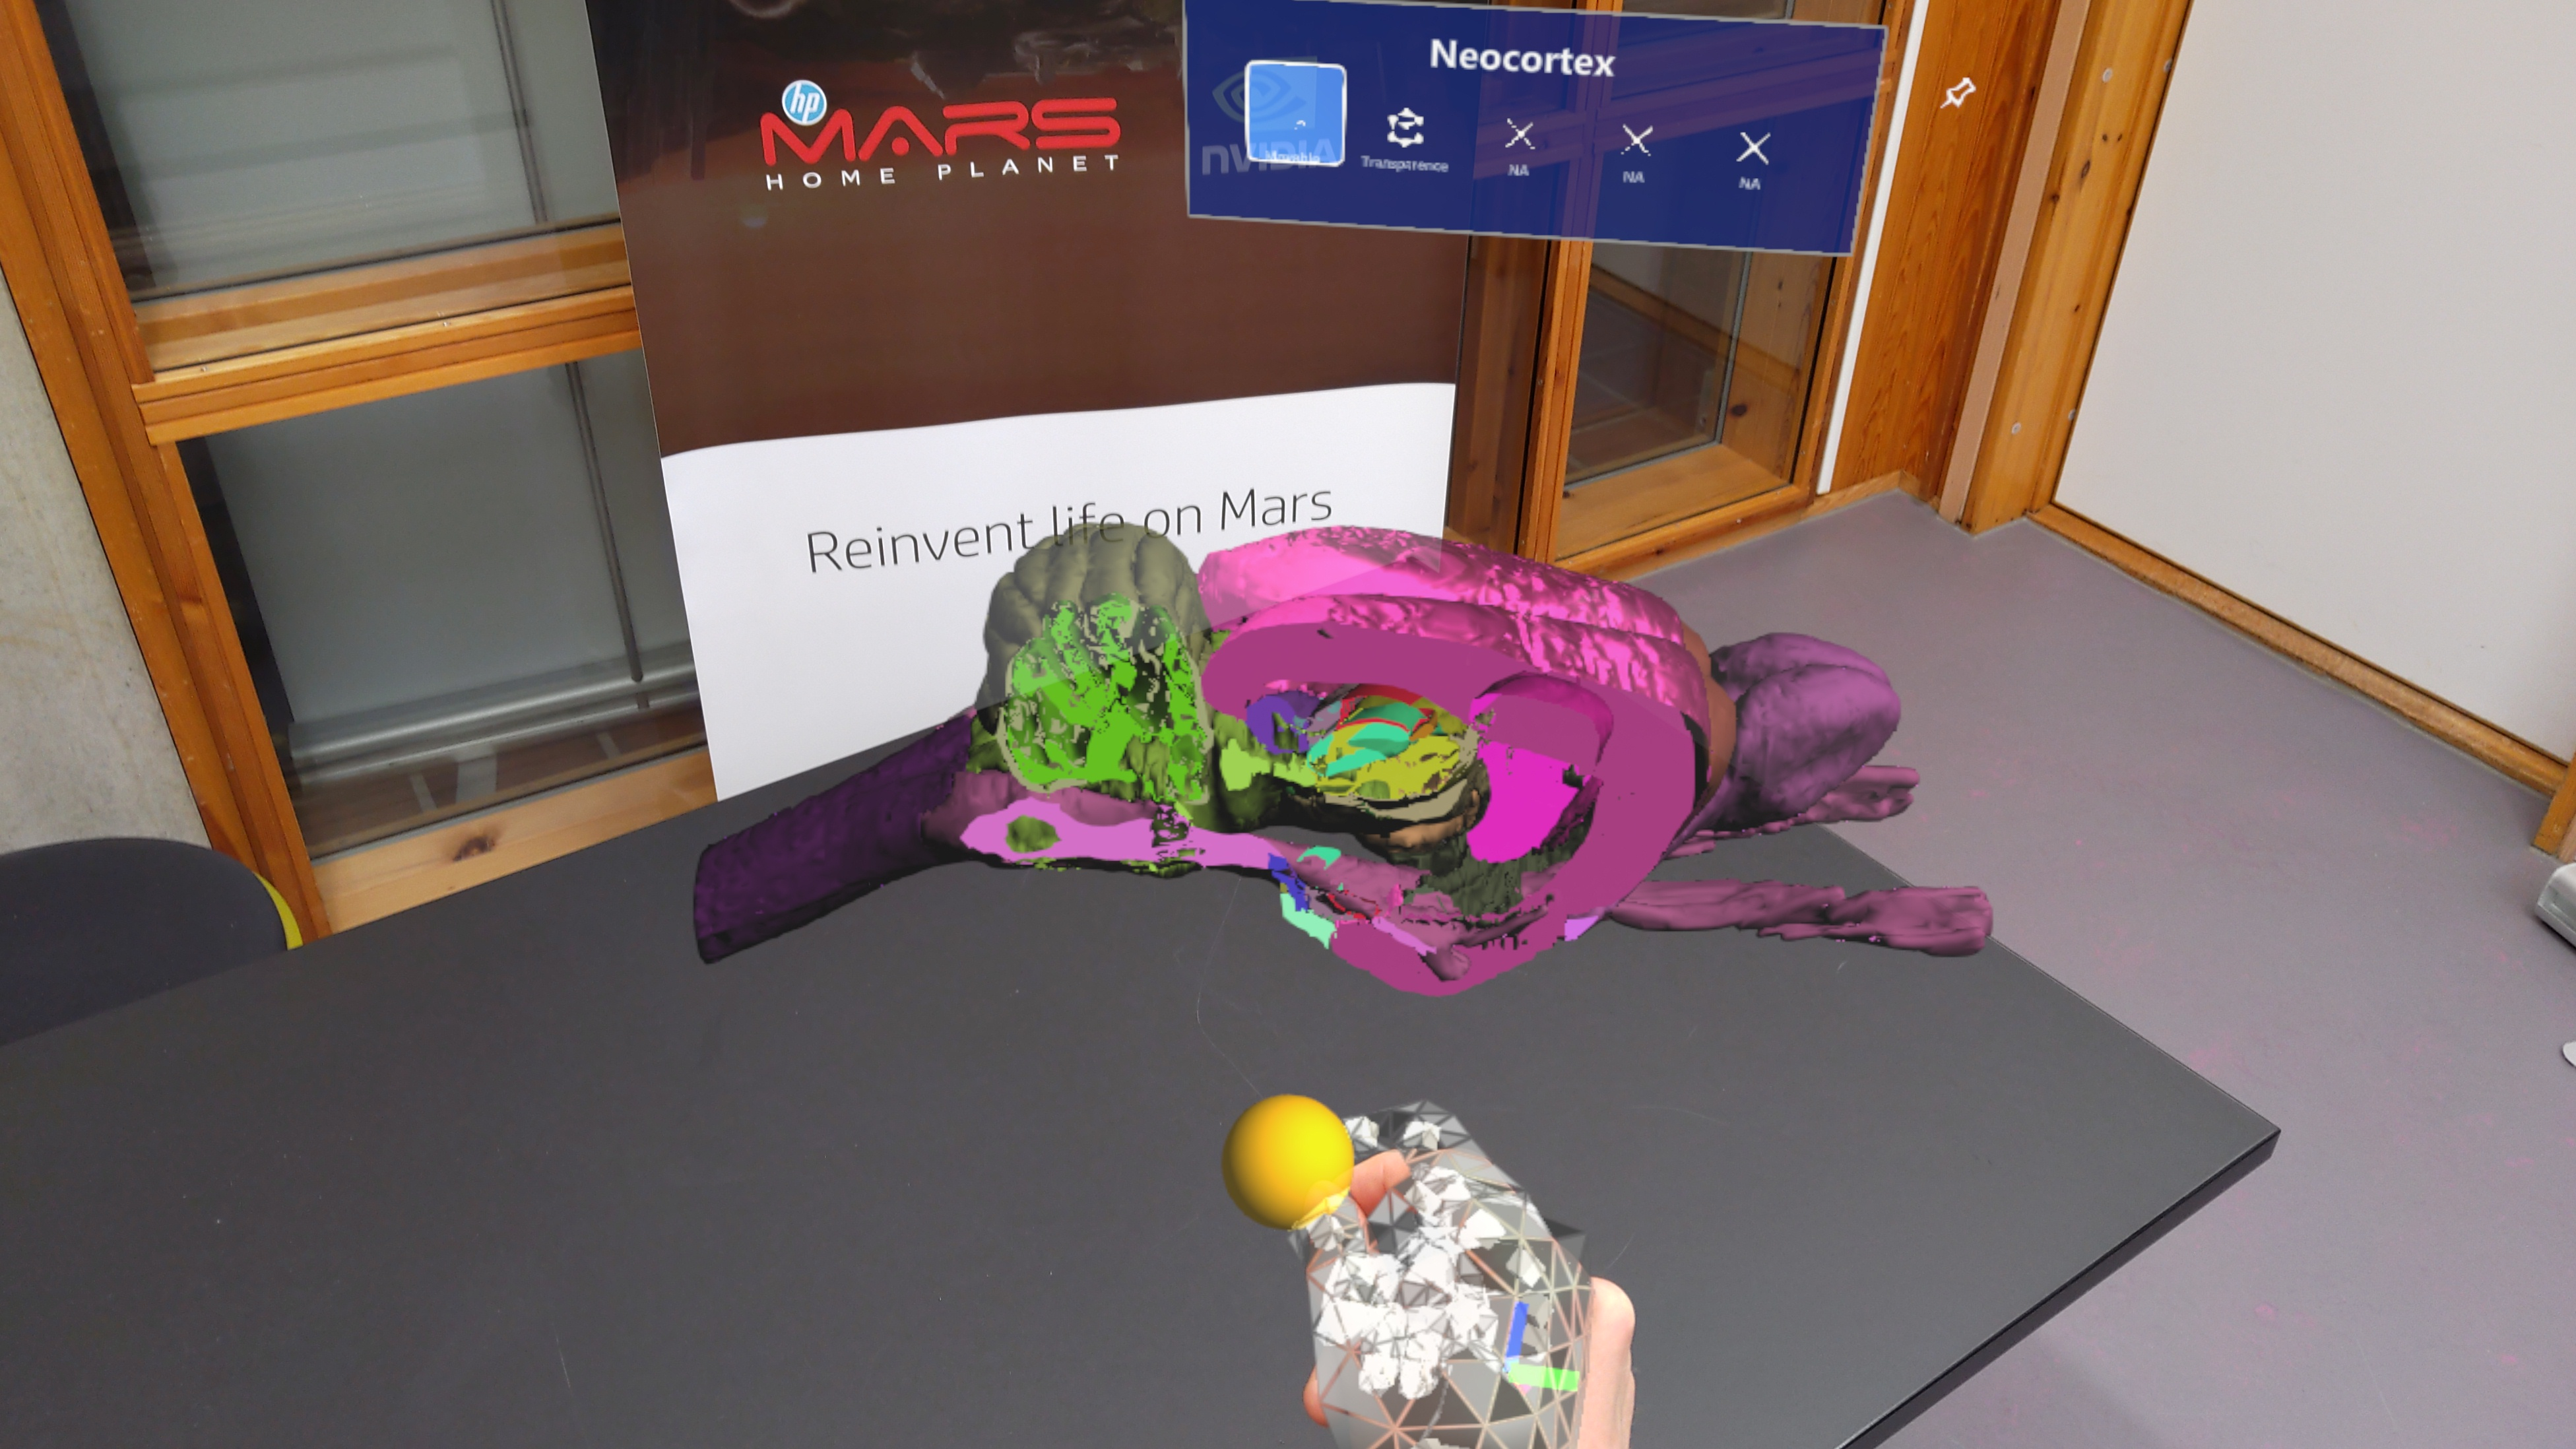
\includegraphics[width=0.5\textwidth]{fig/nevrolens/clipping.jpg}
%     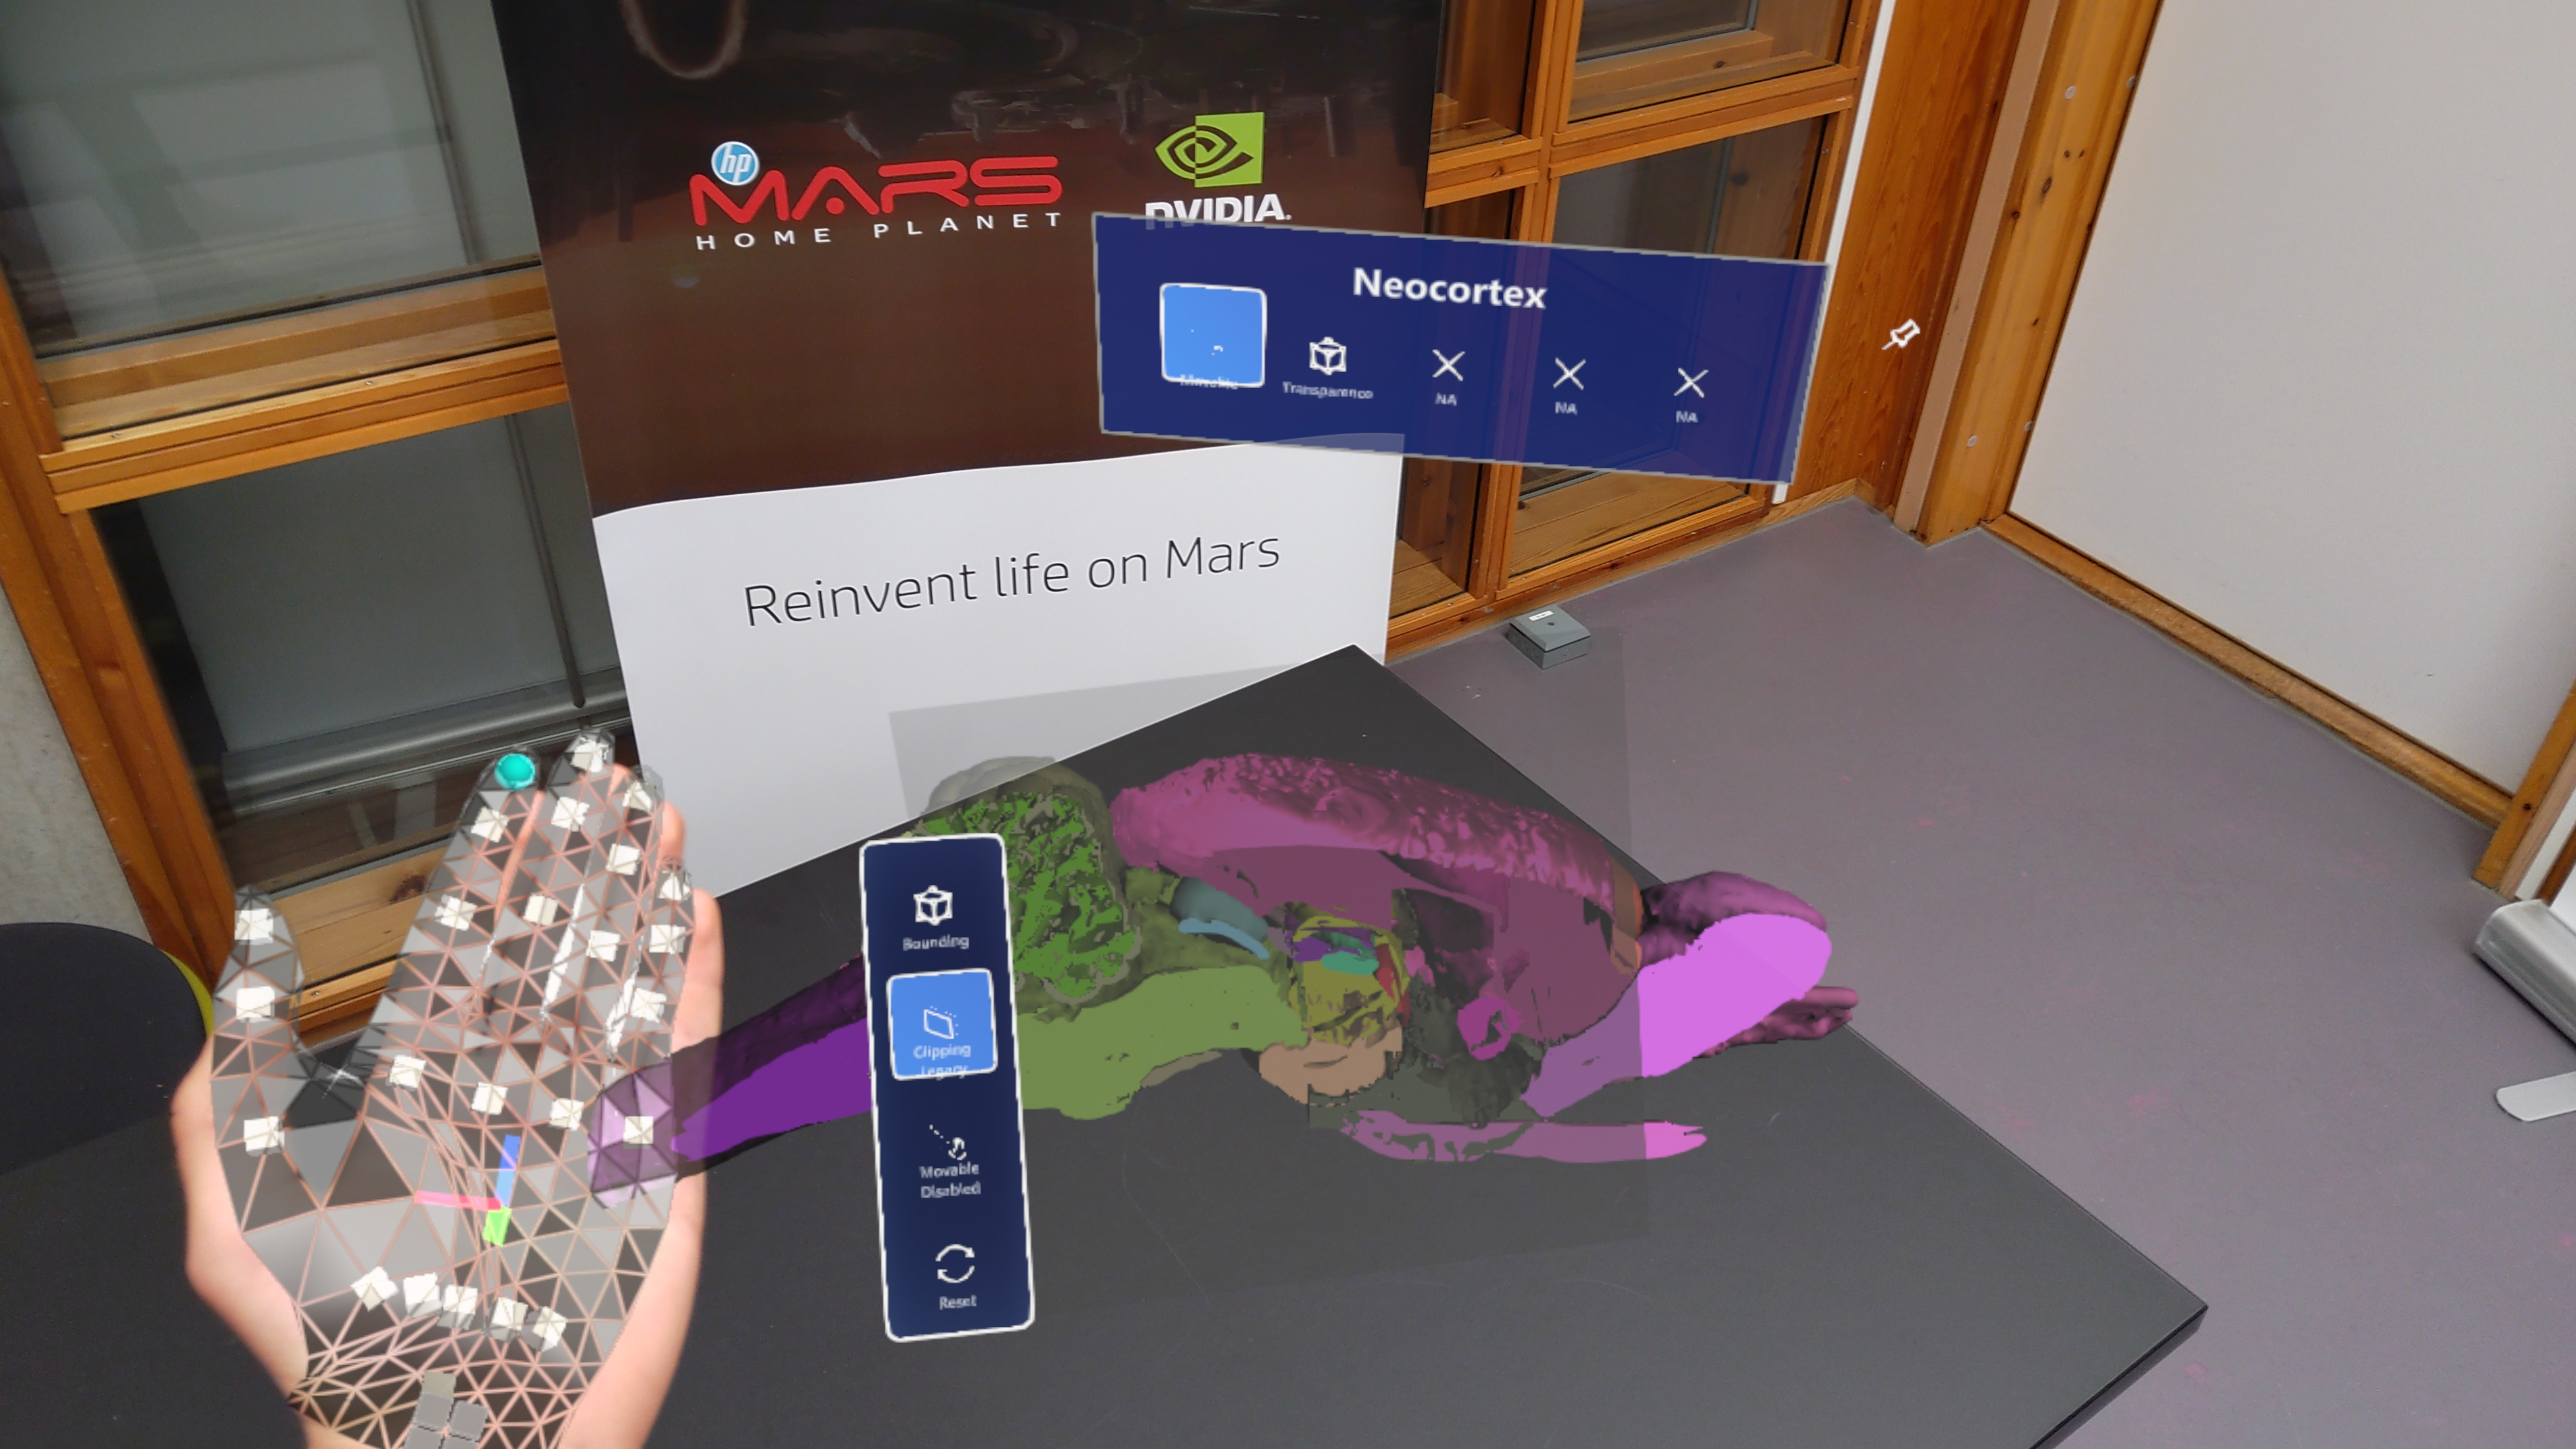
\includegraphics[width=0.5\textwidth]{fig/nevrolens/palmmenu.jpg}
%     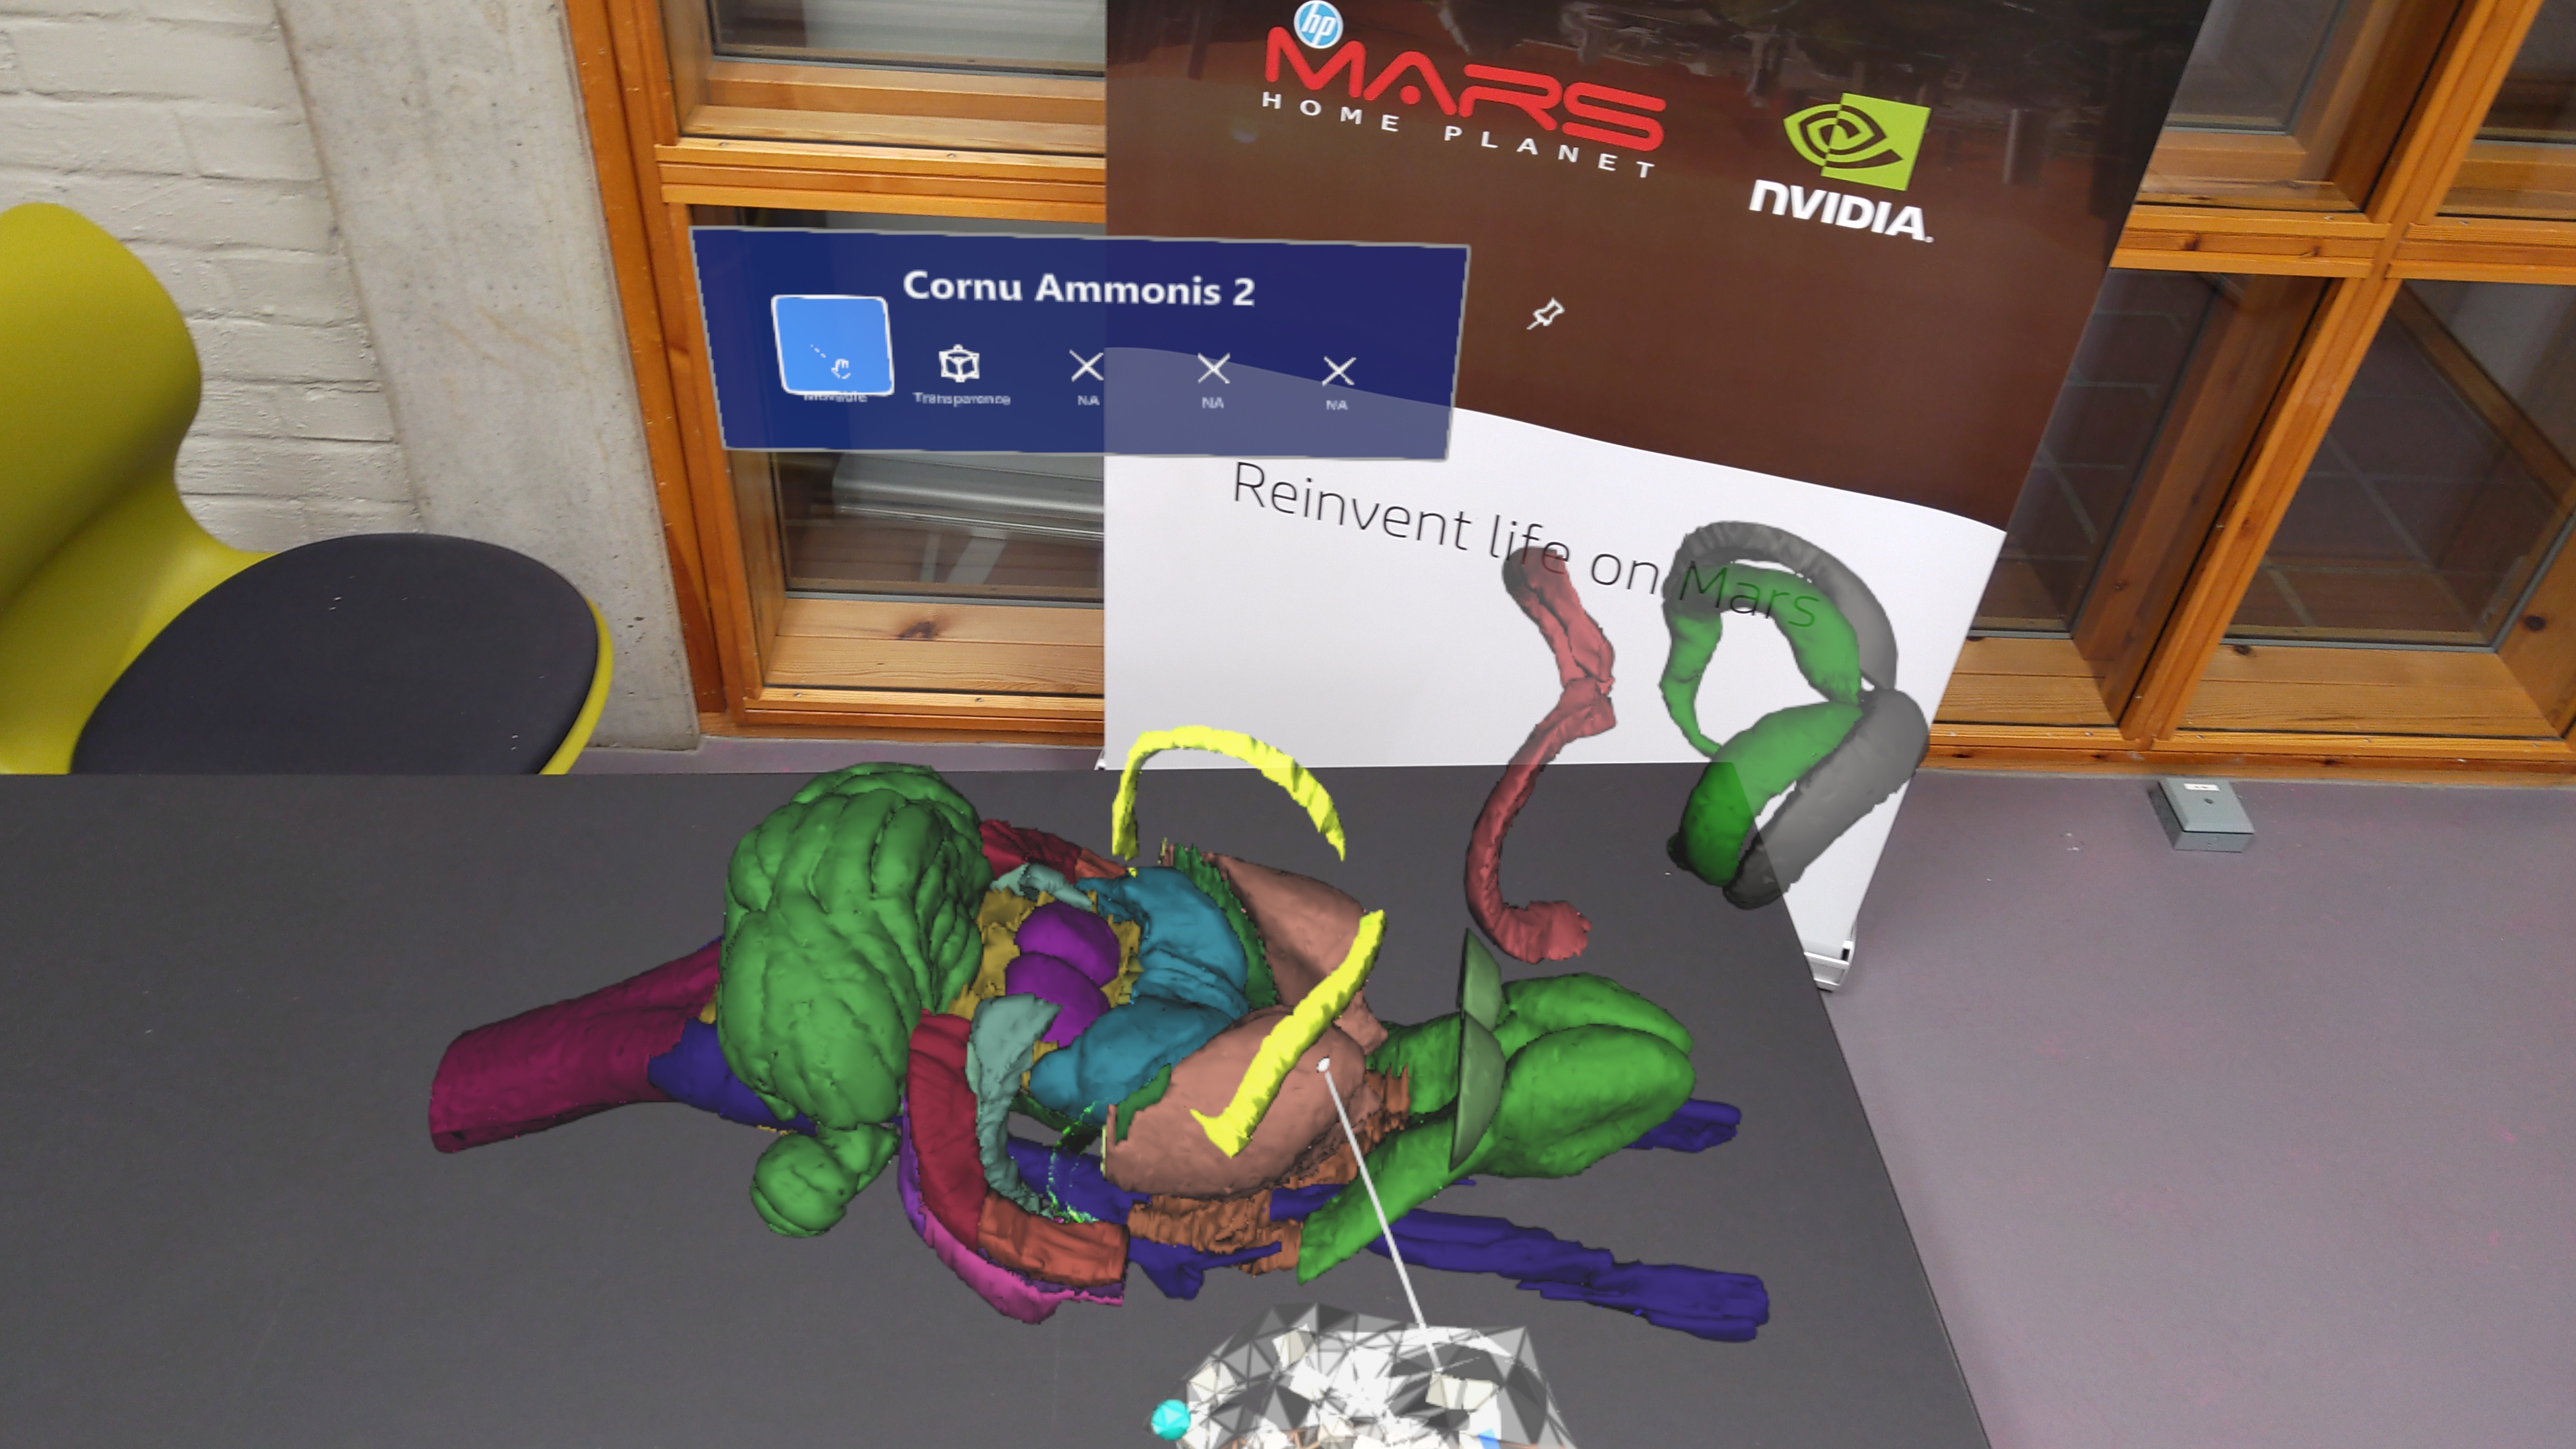
\includegraphics[width=0.5\textwidth]{fig/nevrolens/brainpartsout.jpg}
%     \caption{Nevrolens v0.1.3 on HoloLens 2}
% \end{figure}


% \begin{figure}[h]\label{fig:nevrolens_android}
%     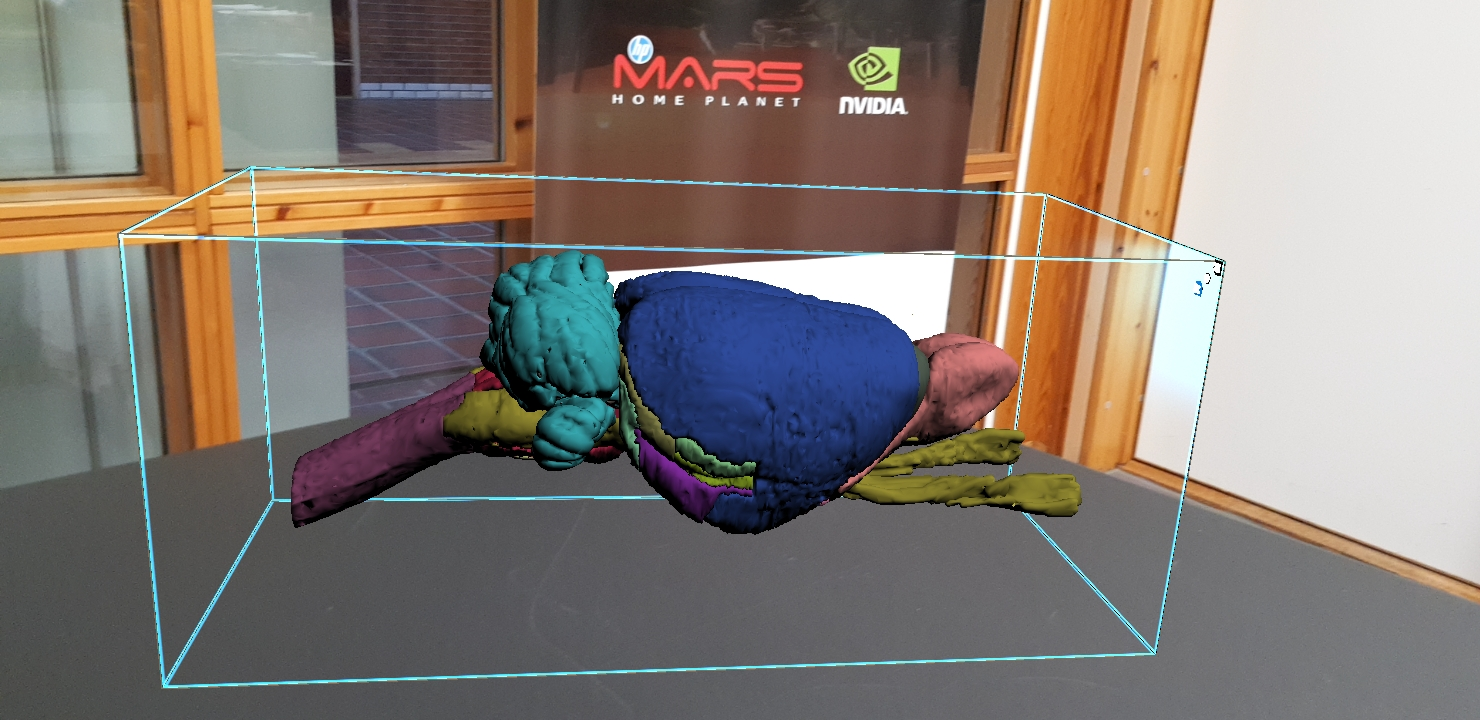
\includegraphics[width=0.5\textwidth]{fig/nevrolens/android_zoom_large.jpg}
%     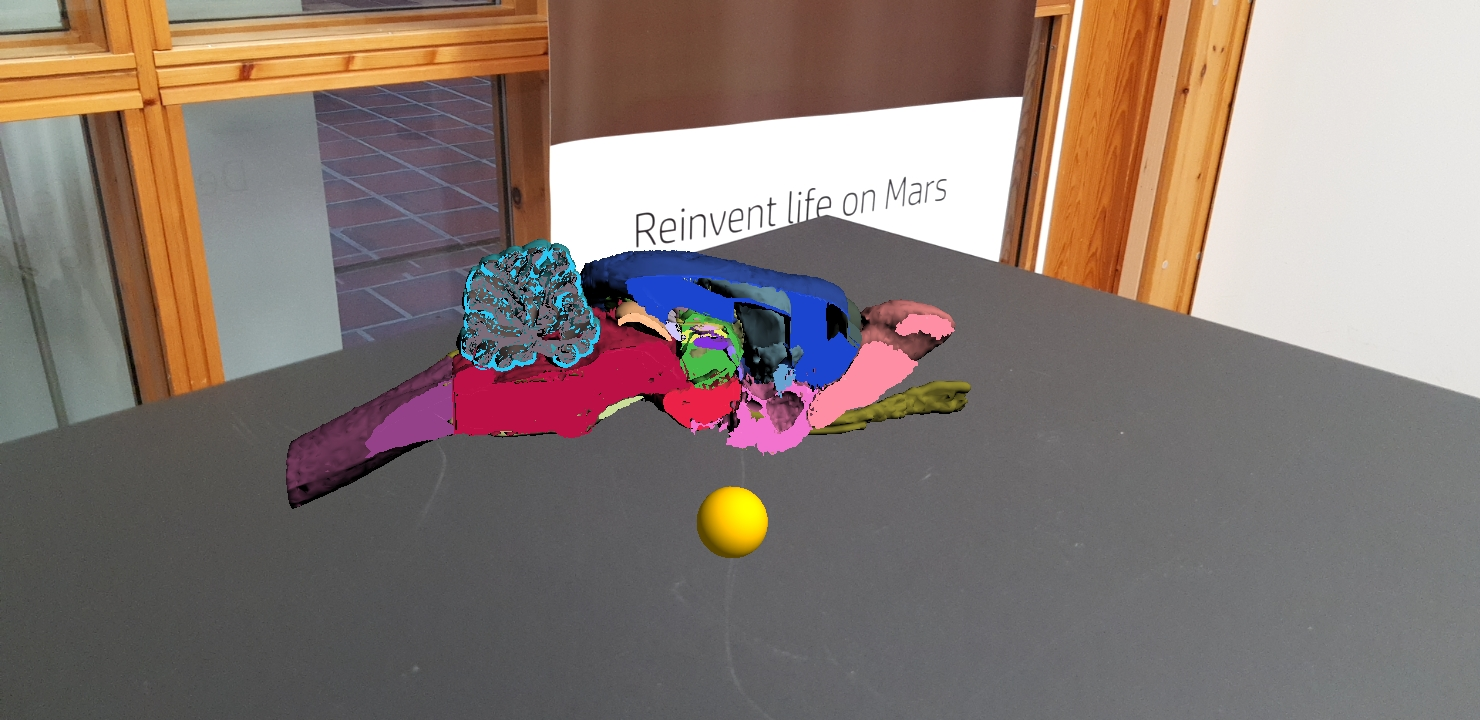
\includegraphics[width=0.5\textwidth]{fig/nevrolens/android_clipping.jpg}
%     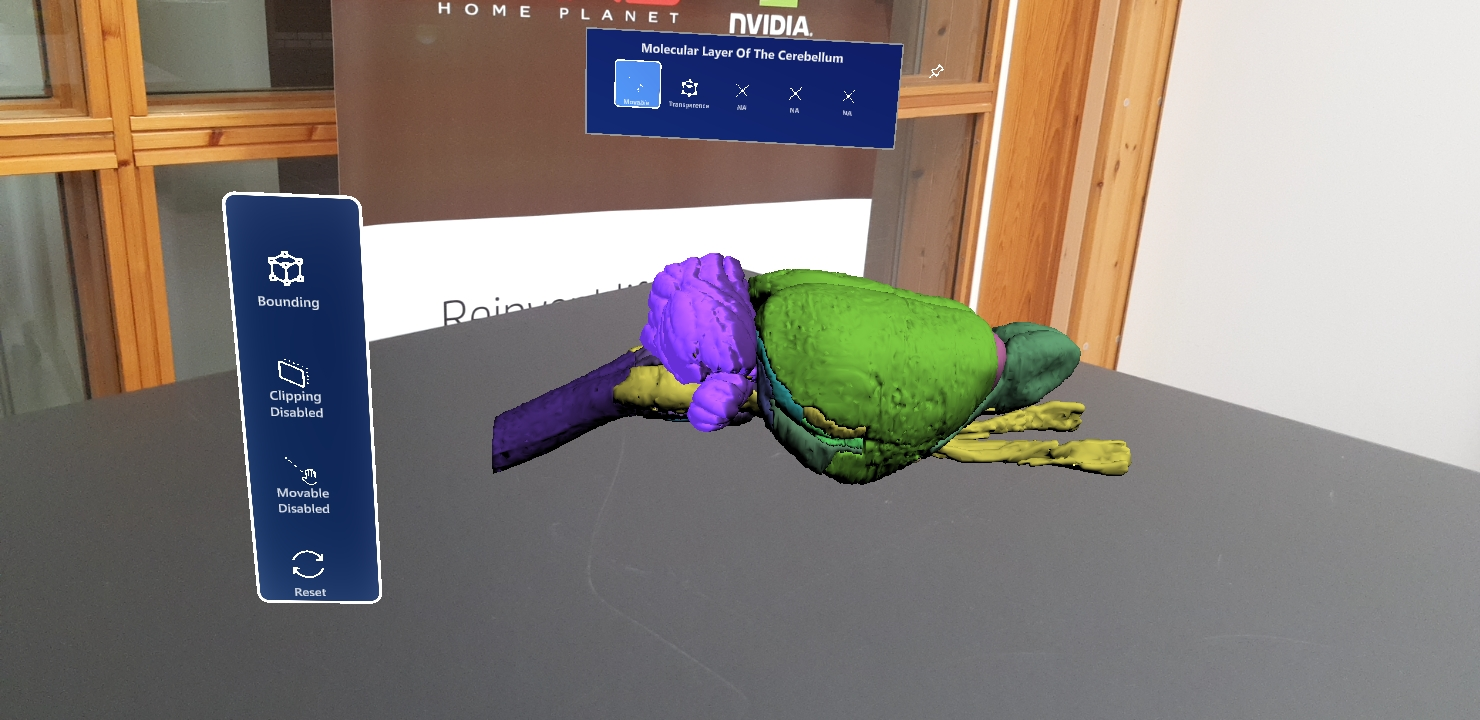
\includegraphics[width=0.5\textwidth]{fig/nevrolens/android_palmmenu.jpg}
%     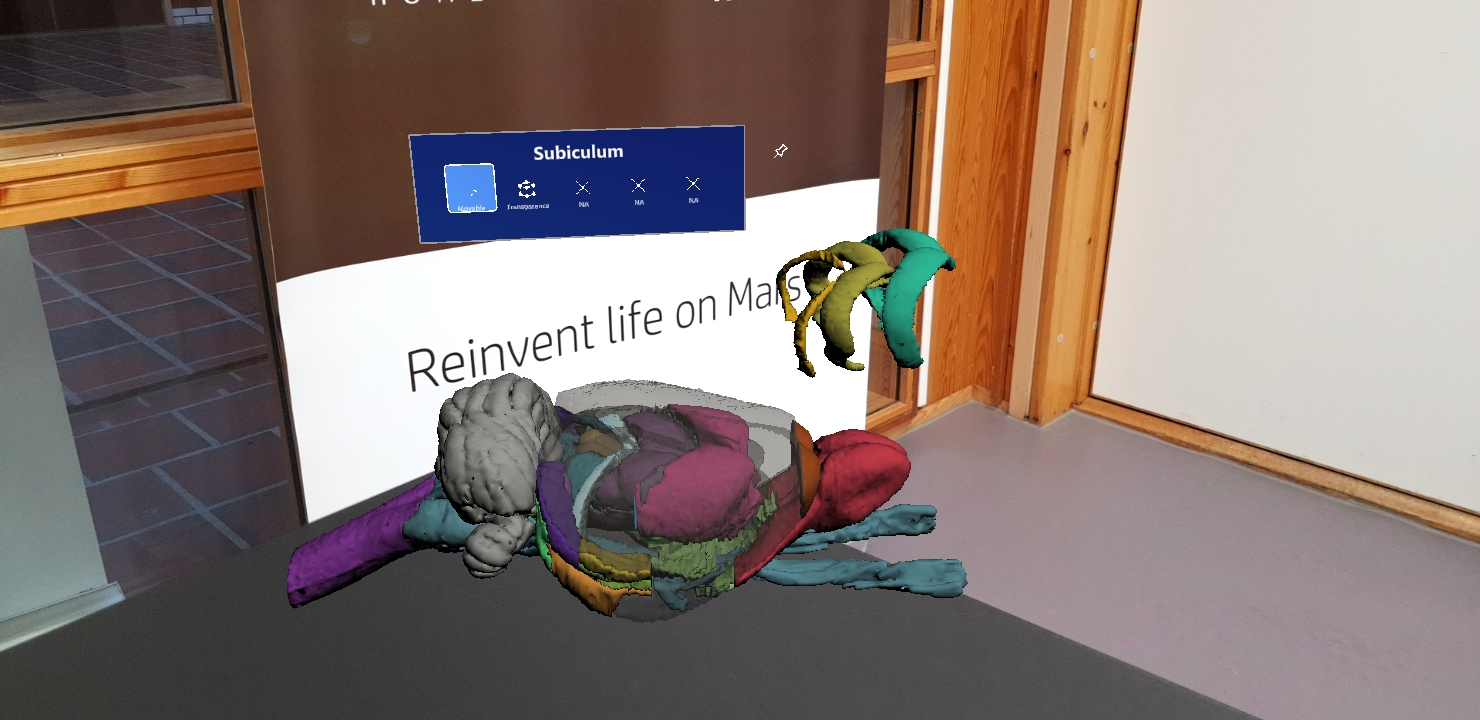
\includegraphics[width=0.5\textwidth]{fig/nevrolens/android_partsout.jpg}
%     \caption{Nevrolens v0.1.3 on Android}
% \end{figure}





% \section{Results}

% Because of the COVID-19 pandemic no user testing has been done this semester, in fact no medical students or professionals have tried the application in-person. Thus, it has been difficult to do formal interviews or gather much feedback, especially regarding interaction. This project is the preliminary work for my master thesis next semester and result gathering will naturally be a much more in focus then. And though no user testing has found place, we have arranged live demoes with \nameref{chap:wdp} over Zoom, which have generated useful feedback. 
% In one such demonstration, I wore a HoloLens 2 and use Nevrolens with guidance from a neuroscientist to extract related regions of the brain and was lectured on their role in behavior. 
% The feedback on its use for a single user, was that there should be a global list menu to toggle different features on each brain part, that there should be ability to increase resolution of a single brain part and some way to visualize microscopical data. 

% % Mostly, the feedback has been positive

% % Success in picking out brain parts, and explaining different structures in the brain. 



% % results from this project are limited.
\chapter{Discussion}

\section{Limitations}

% This project rapport is based on work from a 15 credits course, thus there has been time constraints managing the project with other courses and exams. Combined with the busy schedule of the neuroscientists at the Kavli Institute, it has been challenging to gather feedback in the relatively short time frame of this project.
% Of course, the COVID-19 pandemic has made physical sharing of the headset problematic, and thus user testing has been difficult. 
% In total, there is a very thin basis for results in this project, but this will hopefully be turned around for the master project.


\section{Results}


\section{Hardware limitations}

\subsection{Performance}\label{chap:discussperformance}

The main limiting factor for the performance of the Nevrolens application is the polygon count for the models used. The count for the models uses are around 300,000 for the complete model at decimation ratio 0.08 and an hollow outline model with decimation ration 0.4 at about 350,000 polygons, used in clustering. The counts are higher than what is generally recommended for HoloLens 2, naturally this results in an application which runs well under the best recommended performance quality criteria which the non-functional requirements of this research project set out to meet. The application will hover around 40 to 50 frames per second while in normal use and drop to around 30 to 35 while rendering the volumetric dissection plane, the recommended quality criteria lists 60 fps as a goal for \textit{Best} performance, but the application follows the \textit{Meets} criteria, which state that:
\begin{quote}
\textit{The app has intermittent frame drops not impeding the core experience, or FPS is consistently lower than desired goal but doesn’t impede the app experience.}
\end{quote}
Thus, the application can be said to meet the quality criteria set by Microsoft. 
Throughout testing, framerate was genuinely not a detectable issue, no user tester did at any time commented on low performance and even testers experienced with HoloLens and AR technology did not unprompted notice the low framerate while using the application. This could be the result of the somewhat blurry display of the HoloLens 2, or simply that targeting 60 fps is far less critical in AR application, than in on VR devices. 
On tested Android devices performance has not been of any concern, running at a consistent 60 fps all the time. The teste device is a Samsung Galaxy S8, which was released in 2017 way before the HoloLens 2, and does in fact have a slower processing unit than the HoloLens 2 does. Answering why this performance gap exist will only be speculation, and will not be attempted.
In conclusion, the performance of the application is at an acceptable level and does not impede the user experience, if that were to happen, either by increased load from demanding features or porting to less performant platforms, a natural and easy solution would be to scale down the brain model further.


\subsection{HoloLens 2}

% Because of it being  a see-through display right in front of the uses 
The HoloLens 2 uses a see-through holographic display technology based on a combination of waveguides and light projectors\footnote{https://docs.microsoft.com/en-us/hololens/hololens2-display}, this is a unique display technology developed by Microsoft. This results in images being less sharp and less color accurate than with conventional LCD or OLED displays. From the researchers experience it can be a person to person difference the experience of these issues, the researcher sees the display as muddy, while others have reported not such problem. The display issues are very noticeable when comparing between devices. The first HoloLens 2 device arrived at the VRLab in early spring of 2020, while the second device arrived in April 2021. The old display is even less sharp and color accurate than the newer device.
The consequence of these issues are that high fidelity details on surface models are being washed out and almost indistinguishable from their low fidelity variants. Anecdotally, the researcher, after getting used to seeing the brain models through the HoloLens 2 display got supported by the level of detail observed when outputting the same model on a LCD display from a workstation computer. From the researchers view striving for higher resolution 3D models when rendered on current display technology for AR (HoloLens 2 specifically) is a futile effort.
As discussed in \autoref{chap:discussperformance}, the HoloLens 2 is remarkably less performant than the tested Android handset, when running the research artifact. This is probably a result of poor optimization in the pipe line from building on Unity, through complication in Visual Studio to the HoloLens 2, undoubtedly the Android build pipe line is better optimized as a result of it being a more mature platform.

\subsection{Android}

The main limitation of using Android in this project is that is simply not designed for the purpose. Android devices, like the Samsung Galaxy S8, are design for interaction through touch sensitive displays and not as a viewport for interaction with the wider world. From the test session with the Android application a common feedback was to just disable the AR and have it be more pure experience for Android interaction. This is quite sensible and should definitively be looked further into. The researcher sees to main problems with the approach taken when implementing AR on Android handsets. First, the spatial locking is very poor, resulting in the brain model and other objects moving from their places position during use of the application. This does not meet Microsoft's App quality criteria for holographic stability, rather as the failed criteria states; \textit{Primary content in frame shows unexpected movement}. This may be a device specific issue, as the application has only been tested at reasonable extent on the Samsung Galaxy S8.
The second main problem with Android is that, as mentioned before, interaction on Android handsets is a completely different paradigm from the one of head mounted devices like  HoloLens 2. This means that all UI elements should be platform specific or at least optimized such that they bring good user experience to all platforms. This has not been done during this research project, as the application is now Android users have a considerably poorer experience when interacting with UI than what HoloLens 2 user have. 
Both problems could in the future be solved with stereoscopic rendering, which splits the display in two distinct areas for each eye such that the smartphone when mounted to the head, with specials googles, could simulate the experience of using a HMD device. As current versions of Androids AR API do not support hand tracking, the addition of either third-party APIs like \href{https://www.manomotion.com}{ManoMotion}, or accessories like the Leap Motion controller should be explored. Stereoscopic rendering is as of the time or writing not supported in MRTK, hopefully this will change when Android support gets out of beta. 


\section{Missing data set}
The brain model data set used in this research, which as described in \autoref{chap:zeroiter} was imported from \nameref{chap:vrvis}, is missing a number of brain structures. The model consists of 29 separate structures while the Waxholm Space Rat Brain model it is based on included as least 75 structures. This is of course a huge discrepancy, but it is not as critical as it could seem as most of the omitted structures are very small and would be impractical to handle within AR. Upon questioning Elden has explained that the reduction was done to decrease computational time as the model was meant for a proof of concept. As this is still the case the reduces number of brain structures is still not a critical issue, however if this research project were to be used as an actual educational tool this would be of most dire need for fixing. Another reason this issue has not seen any need for fixing is that there will be a new version of the Waxholm Space brain model released shortly, and stakeholders at Kavli are interested in the use of this model in further research, thus creation of a new brain model has been deferred to \nameref{chap:futurework}. A increases in structure count could however result in increased polygon count which would have to be accounted for then scaling the resolution of the surface models.

% There is however one quite notable structure missing, the \textit{Corpus Collosum} .
\section{Human neuroanatomy}
% Describe/explore the feasibility to implement the system for Human neuroanatomy education.

The stakeholders of this research from the Kavli Institute expressed interest from the very begin of this project to extend the its functionality to support human neuroanatomy educational. In principle, nothing in this research project sets a limit this from becoming a really. In fact, replacing the WHS rat brain model with a surface model of the human brain could be done with very little effort. In future development, the researcher envisions a system for importing different brain models into the application with limited overhead. 

% This could possibly be done by 
% This is probably something of a pipedream.


% display issues

% \section{Contribution}

% !TEX encoding = UTF-8 Unicode
% !TEX root = ../thesis.tex
% !TEX spellcheck = en-US
%%=========================================
\chapter{Conclusion}




%%=========================================
\section{Limitations}

This project rapport is based on work from a 15 credits course, thus there has been time constraints managing the project with other courses and exams. Combined with the busy schedule of the neuroscientists at the Kavli Institute, it has been challenging to gather feedback in the relatively short time frame of this project.
Of course, the COVID-19 pandemic has made physical sharing of the headset problematic, and thus user testing has been difficult. 
In total, there is a very thin basis for results in this project, but this will hopefully be turned around for the master project.


%%=========================================
\section{Discussion}

% The research question the project set out to answer are


This project has mainly focused on implementing the application answering \href{subrq1}{Sub-RQ1}. As such this can be seen as a minimal viable product for exploring Sub-RQ1, and in that capacity it has shown great promise. The basic tools for dissection is implemented and the medical academics at Kavli Institute and UiO sees great potential in its use. 
As for the Sub-RQ2 and 3, there is less work done. However, by building the application for Android, I have shown that the possibility for cross-platform collaboration is open. And it will be worked on for the master thesis, by implementing networking with \nameref{chap:photon}. Sub-RQ3, has not seen any concrete development, I do have some ideas of how it could be implemented with textures generated from a volumetric brain model. 


%%=========================================
\section{Conclusion}

The state of the project now is a small scale proof of concept for a AR application supporting teaching of neuroanatomy and dissection for medical students. There is still no collaboration or microscopic data visualization in the app. However, the biggest problem with the state of the project is the lack of concrete feedback from medical user groups. It has been received very positively by the neuroscientists who has seen the application in use, and they are awaiting more news on the project. The need for exact user testing and user feedback is still large. The project is however progressing nicely, and with further development I believe this project could create impressing results.


%%=========================================
\section{Further Work}\label{chap:futurework}

% \begin{itemize}
%     \item Collaboration, Networking
%     \item Macro+micro implementation
%     \item Importing new models
%     \item Look into volumetric rendering  
% \end{itemize}

There is still a lot of work left on this project, and it will be continues by me. While there is numerous features and fixes which are waiting in the backlog I would like to focus on the overall picture and what has to be in focus to create an collaborative educational experience in AR. 

\begin{itemize}

    \item {
        \textbf{Focus on usability}\\
        Implement better guidance and affordance such that anyone can use the application. To manage this it will be essential to have user testers and testing with medical user groups. This will give feedback on what makes sense and what doesn't.
        
    }
    \item {
        \textbf{Collaboration; implement cross-platform networking}\\
        Networking tools will be required to create a collaborative experience, this will be done using \nameref{chap:photon} to synchronize the HoloLens 2 application with the Android application.
    }

    \item {
        \textbf{Visualize volumetric data}\\
        While the HoloLens 2 does support volumetric rendering, I am pretty sure it is not in an adequate resolution for this project. It will however be explored. Other than that volumetric data could be used as 2D textures mapped on the clipping plane used to cut the brain.
    }

    \item {
        \textbf{Explore ways of using other brains}\\
        \autoref{chap:elden} explains the steps taken by \citet{Elden2017} to use medical imagery in \nameref{chap:vrvis}. An exploration into whether there is a more elegant way of doing this, should be done.
    }

A general focus when continuing this project should be gathering more user data in the form of user tests and interviews, there should be a focus on establishing whether this project can improve learning outcomes for medical students.


\end{itemize}

\section{Future Work}

% Add newer data set WHS rat brain v4

% Add human brain

% Make app more dynamic => Import brain, labels, infoborad text in runtime

% Improve networking stuff => Microsoft Mesh

% Photon Voice

% Improve Android app => menus with android UI should be possible

% More microscopicaldata Sub RQ3

% Desktop or WebGL view app


This section will lay down suggestions for how to further the project. These are based on the authors experience with the research project and on discussions with the neuro specialists and medical students testing the application.

\subsubsection*{Import new data sets}

As described in \autoref{chap:ratbrain} the WHS rat brain is under continuous development and the the near future there will be released a forth version of the brain model, with improved delineation. It is a high priority wish from the Kavli Institute to use this brain model in the application.

To import a WHS brain model as a geometric model is a complicated process, which has been explained by Elden in \autoref{chap:elden}.
The process of exchanging the geometric model used now with a new one however is trivial, but time consuming. A considerable improvement to the application would be the ability to drop in a new model, preferable at run time such that the application wouldn't need to be build and deploy for each model change.
This would enable future WHS versions to easily be added and even other models like human brains could be switched between.  

Another essential feature to reduce the need for new builds is to enable configuration in-app. The application uses three different text files which saves the configuration of clustering, infoboard and labels, all of these should either be possible to upload at run time or configuration with settings UI in-app.

\subsubsection*{Improve networking}
A critical improvement to the application would be to have the initial scene of the application give the user an option of creating a room, joining an existing room or playing offline.
The application as of now will automatically behind the scene, join the existing room or create one if there is none. This gives users less control but more frictionless when testing collaborative features. In a full scale application the user control would probably be preferable.

The networking solution in the application has a considerable amount of bugs and unexpected behavior, this is probably something that is difficult to completely circumvent, but an effort to restructure or fix this should be done.

%todo Microsoft Mesh?

\subsubsection*{Voice chat}

When collaborating in-app remotely the ability to talk to each other would be a great feature, which for a full scale application would be a high priority. 
This can be done with by using Photon Voice for PUN 2.

\subsubsection*{Platform specific input and UI}
There are few limitations in which platforms the application can run on. However, each platform comes with it's own needs for specific input types and UI. The application has been always been developed with HoloLens 2 as the highest priority and that can be seen in most choices taken conserving UI and input handling. Increasing the user experience on Android and even Windows or WebGL (the application is buildable for both, but needs input handling to be usable) should be a priority. Feedback from user testers gave indication that the augmented reality in the android version did not provide an improved user experience and thus disabling camera and spatial features in Android could be seen as an improvement, which could be extended to a desktop application.
A future version of the application running on the web, with WebGL, would probably be possible and further the goal of accessibility.











% Include more chapters as required.
%%=========================================
\appendix
% !TEX encoding = UTF-8 Unicode
%!TEX root = thesis.tex
% !TEX spellcheck = en-US
%%=========================================

\chapter{Acronyms}
\begin{description}
\item[NTNU] Norwegian University of Science and Technology
\item[AR] Augmented Reality
\item[MR] Mixed Reality
\item[XR] Extended Reality
\item[VR] Virtual Reality
\item[HMD] Head-mounted display
\item[WHS] Waxholm Space
\item[GPU] Graphics Processing Unit
\item[SDK] Software Development Kit
\item[COVID-19] Coronavirus Disease 2019
\end{description}
% !TEX encoding = UTF-8 Unicode
%!TEX root = thesis.tex
% !TEX spellcheck = en-US
%%=========================================

\chapter{A geometric model of the rat brain}\label{chap:elden}

This is a section from \citet{Elden2017}, the master thesis about \nameref{chap:vrvis} the VR application this project is loosely inspired by. The section explains how Elden extracted a geometric model of the rat brain from the medical models which is high fidelity volumetric data. I have included it in this report because it gives insight into a specific solution to a problem I face and it explains how a resource I use in this project was created.

\section*{5.2 Exporting segments of a rat brain atlas as geometry
for the Rat Brain model}
The geometric meshes used for the rat brain model were extracted from
a volumetric and segmented atlas. IKT-SNAP was used to export each
segment of the brain as an STL file. These geometric meshes were then
opened in Blender3
to be converted to OBJ or FBX files. 3DS Max imported
the models and performed all modifications made to the geometry and
structure.
ITK-SNAP requires three files to segment and label the models; the
atlas and a segmentation file, both stored as NII files, and a LABEL file
for the labels. When all files are loaded the program lets the user select a
segment to export and generate a geometric hull along the boundary of the
segment. Due to instability experienced with 3DS Max using all 16 GB of
RAM available on the computer used for development, Blender was used
to first convert the files to FBX files. These FBX files caused no issues when
imported into 3DS Max. Since these meshes were too detailed, they needed
to be reduced and transformed in 3DS Max. The meshes were reduced
such that the entire model consisted of 4.5 million triangles. Most of the
meshes had to be transformed such that each segment was where it should
be inside the model. For some reason the exported meshes were of several
relative scales and heights and a lot of manual work went into moving
and scaling the meshes to match the volumetric model seen in ITK-SNAP.
Properly processed, the model was exported as an FBX file and sent to UE4.

\chapter{Neuroanatomy test}\label{chap:knowtest}
\chapter{Nevrolens Questionnaire}\label{chap:questionnaire}


\newpage
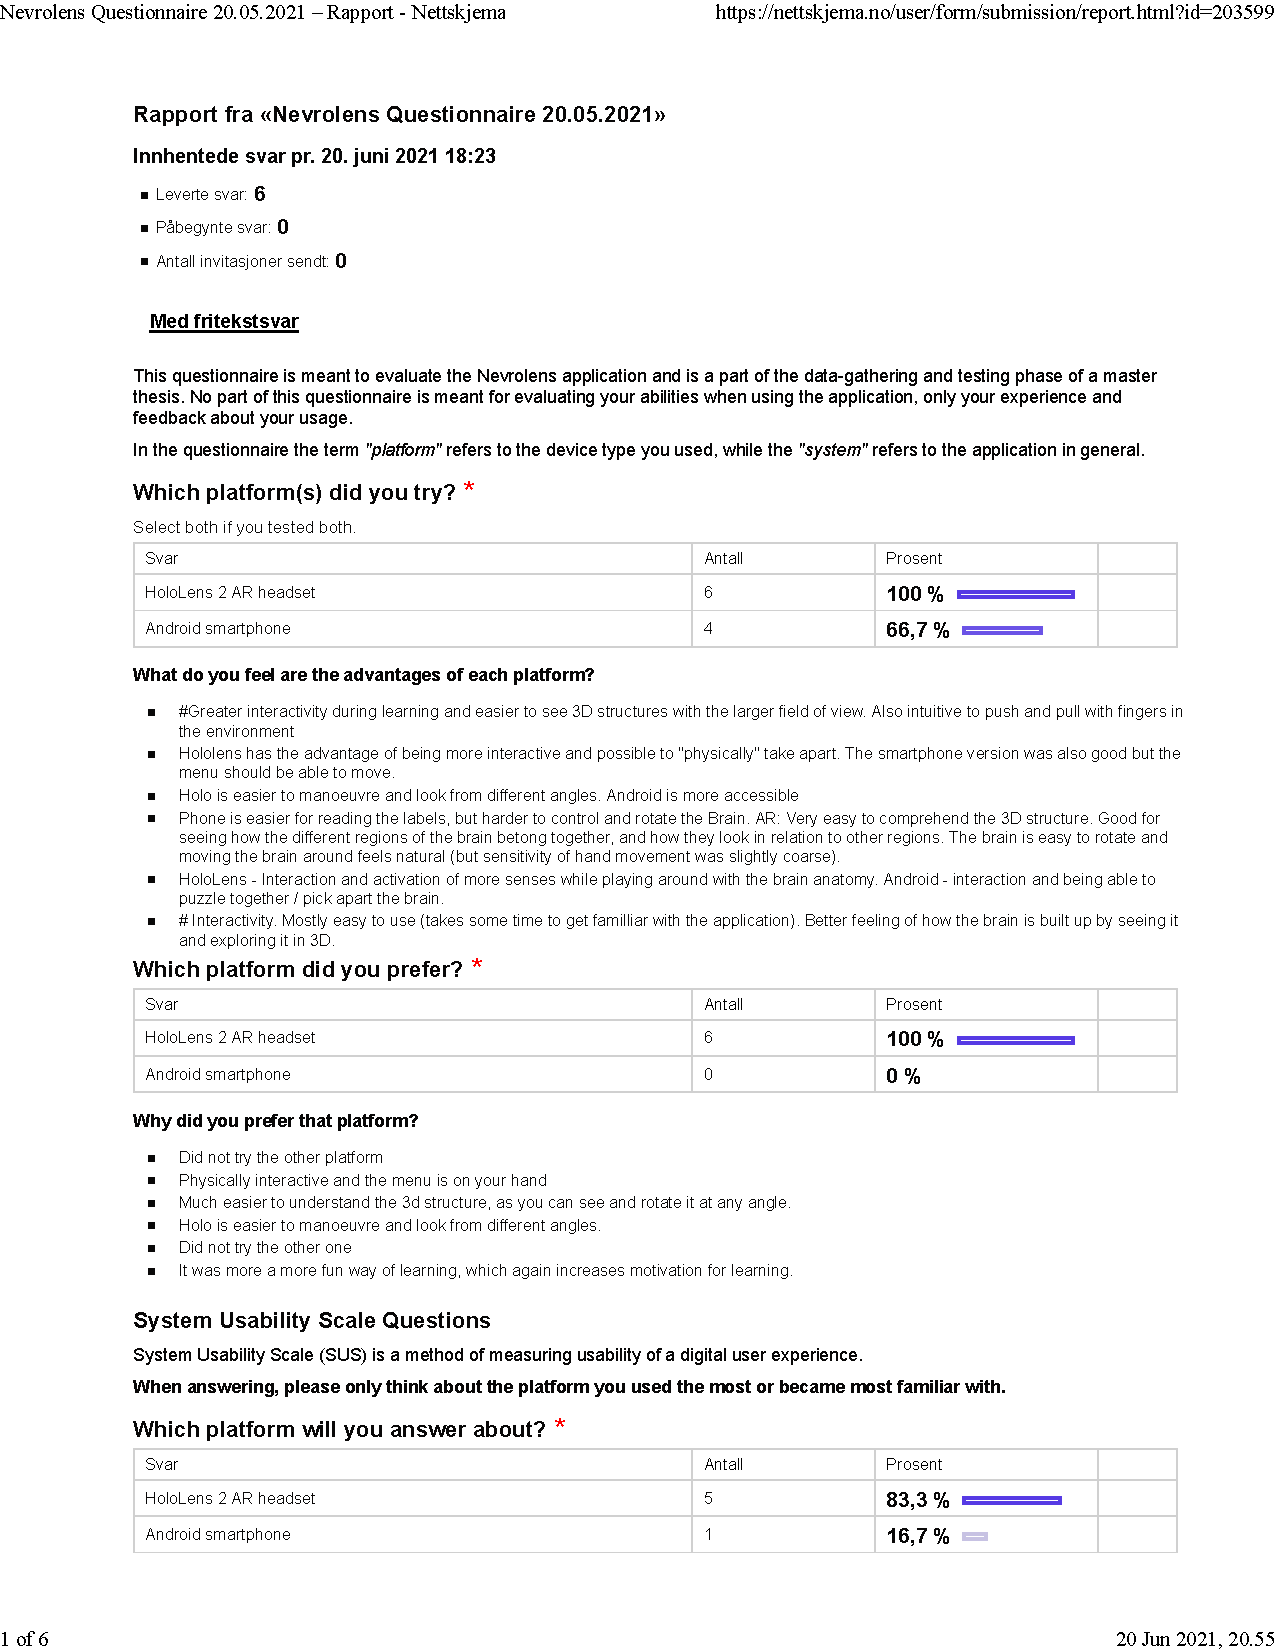
\includepdf[pages=-]{appendix/questionnaire_answered}
% Include more appendices as required.
%%=========================================
\bibliographystyle{apa}
\addcontentsline{toc}{chapter}{\bibname}
\bibliography{refs}  
%%=========================================
%% !TEX encoding = UTF-8 Unicode
%!TEX root = thesis.tex
% !TEX spellcheck = en-US

%This is the Curriculum Vitae
%%=========================================
\addcontentsline{toc}{chapter}{Curriculum Vitae}
\chapter*{Curriculum Vitae}
\hrule
\begin{minipage}[t]{0.65\linewidth}
\begin{tabular}{ll}
Name: & \textbf{Your Name}\\
Gender: & Female\\
Date of birth: & 1. January 1995\\
Address: & Nordre gate 1, N--7005 Trondheim \\
Home address: & King's road 1, 4590 Vladivostok, Senegal\\
Nationality:    & English \\
Email (1): & your.name@stud.ntnu.no\\
Email (2): & yourname@gmail.com\\
Telephone: & +47 12345678\\
\end{tabular} 
\end{minipage}\hfill
\begin{minipage}[t]{0.25\linewidth}
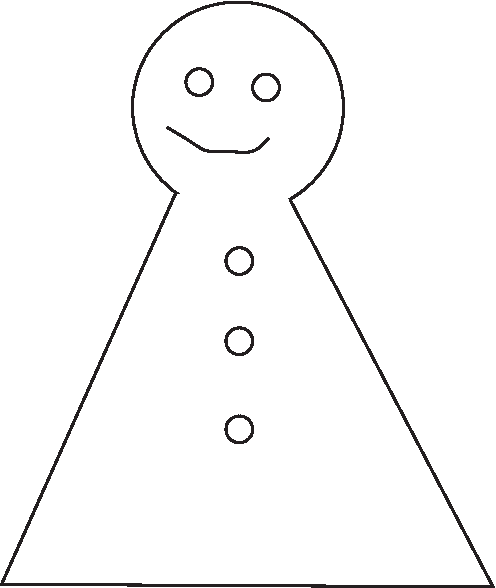
\includegraphics[scale=0.3]{fig/me}\\[1pc] Your picture
\end{minipage}
\hrule

%%=========================================
\section*{Language Skills}
Describe which languages you speak and/or write. Specify your skills in each language.

%%=========================================
\section*{Education}
\begin{itemize}
\item School 1
\item School 2
\item School 3
\end{itemize}

%%=========================================
\section*{Computer Skills}
\begin{itemize}
\item Program 1
\item Program 2
\item Program 3
\end{itemize}

%%=========================================
\section*{Experience}
\begin{itemize}
\item Job 1
\item Job 2
\item Job 3
\end{itemize}

%%=========================================
\section*{Hobbies and Other Activities}         % Your curriculum Vitae     
%%=============================================

\end{document}
